\ifx\wholebook\relax \else
\documentclass[b5paper]{article}
\usepackage[nomarginpar
  %, margin=.5in
]{geometry}

\addtolength{\oddsidemargin}{-0.05in}
\addtolength{\evensidemargin}{-0.05in}
\addtolength{\textwidth}{0.1in}
\usepackage[en]{../../prelude}

\setcounter{page}{1}

\begin{document}

\title{Quick sort and merge sort}

\author{Xinyu~LIU
\thanks{{\bfseries Xinyu LIU} \newline
  Email: liuxinyu95@gmail.com \newline}
  }

\maketitle
\fi

\markboth{Quick sort and merge sort}{Elementary Algorithms}

\ifx\wholebook\relax
\chapter{Quick sort and merge sort}
\numberwithin{Exercise}{chapter}
\fi

\section{Introduction}
\label{introduction}

People proved the performance upper limit be $O(n \lg n)$ for comparison based sort\cite{TAOCP}. This chapter gives two divide and conquer sort algorithms: quick sort and merge sort, both achieve $O(n \lg n)$ time bound. We also give their variants, like natural merge sort, in-place merge sort, and etc.

\section{Quick sort}
\index{Quick sort}

\begin{figure}[htbp]
 \centering
 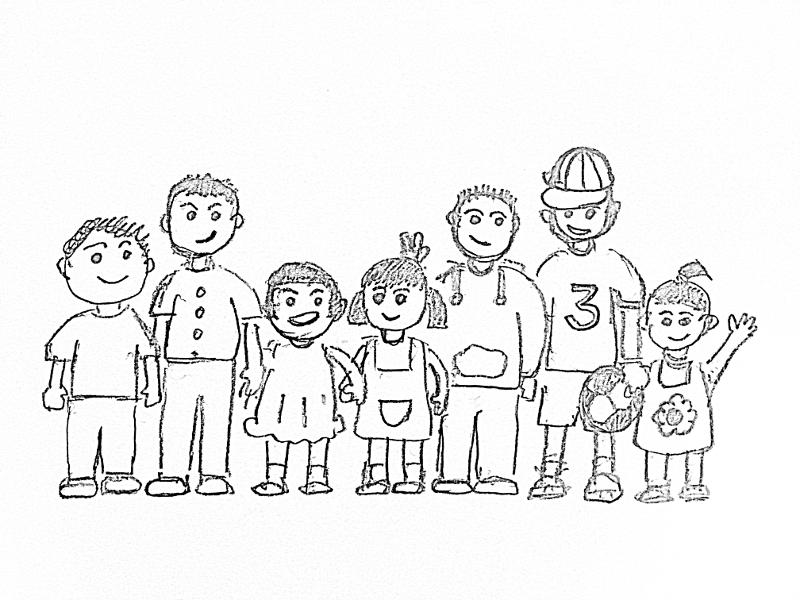
\includegraphics[scale=0.3]{img/kids}
 \captionsetup{labelformat = empty}
 \label{fig:knuth-ssort}
\end{figure}

Consider arrange kids in a line ordered by height.

\begin{enumerate}
\item The first kid raises hand, all shorter one move to left, and the others move to right;
\item All kids on the left and right repeat.
\end{enumerate}

For example, the heights (in cm) are $[102, 100, 98, 95, 96, 99, 101, 97]$. Table \ref{tab:kids-sort} gives the steps. (1) The kid of 102 cm raises hand as the pivot (underlined in the first row). It happens the tallest, hence all others move to the left as shown in the second row in the table. (2) The kid of 100 cm is the pivot. Kids of height 98, 95, 96, and 99 cm move to the left, and the kid of 101 cm move to the right, as shown in the third row. (3) The kid of 98 cm is the left pivot, while 101 cm is the right pivot. Because there is only one kid on the right, it's sorted. Repeat this to sort all kids.

\begin{table}[htbp]
\centering
\begin{tabular}{ | c c c c c c c c |}
\hline
\underline{102} & 100 & 98 & 95 & 96 & 99 & 101 & 97 \\
\underline{100} & 98 & 95 & 96 & 99 & 101 & 97 & `102' \\
\underline{98} & 95 & 96 & 99 & 97 & `100' & 101 & `102' \\
\underline{95} & 96 & 97 & `98' & 99 & `100' & `101' & `102' \\
`95' & \underline{96} & 97 & `98' & `99' & `100' & `101' & `102' \\
`95' & `96' & 97 & `98' & `99' & `100' & `101' & `102' \\
`95' & `96' & `97' & `98' & `99' & `100' & `101' & `102' \\
\hline
\end{tabular}
\caption{Sort steps}
\label{tab:kids-sort}
\end{table}

We can summarize the quick sort definition, when sort list $L$:

\begin{itemize}
\item If $L$ is empty$[\ ]$, the result is $[\ ]$;
\item Otherwise, select an element as the pivot $p$, recursively sort elements $\leq p$ to the left; {\em and} sort other elements $> p$ to the right.
\end{itemize}

We say {\em and}, but not `then', indicate we can parallel sort left and right. C. A. R. Hoare developed quick sort in 1960\cite{TAOCP}\cite{wiki-qs}. There are varies of ways to pick the pivot, for example, always choose the first element.

\be
\begin{array}{rcl}
sort\ [\ ] & = & [\ ] \\
sort\ (x \cons xs) & = & sort\ [y | y \in xs, y \leq x] \doubleplus [x] \doubleplus sort\ [y | y \in xs, x < y] \\
\end{array}
\ee

We use the Zermelo Frankel expression (ZF expression)\footnote{Name after two mathematicians found the modern set theory.}. $\{ a | a \in S, p_1(a), p_2(a), ... \}$ selects elements in set $S$, that satisfy every the predication $p_1, p_2, ...$ (see chapter 1). Below is example code:

\lstset{frame = single}
\begin{Haskell}
sort [] = []
sort (x:xs) = sort [y | y<-xs, y <= x] ++ [x] ++ sort [y | y<-xs, x < y]
\end{Haskell}

We assume to sort in ascending order. We can abstract the comparison to sort different things like numbers, strings, and etc. (see chapter 3) We needn't total ordering, but at least need {\em strict weak ordering}\cite{wiki-total-order}\cite{wiki-sweak-order}(see chapter 9). We use $\leq$ as the abstract comparison.

\subsection{Partition}
\index{Quick sort!partition}
We traverse elements in two passes: first filter all elements $\leq x$ ; next filter all $> x$. We can combine them into one pass:

\be
\begin{array}{rcl}
\textit{part}\ p\ [\ ] & = & ([\ ], [\ ]) \\
\textit{part}\ p\ (x \cons xs) & = & \begin{cases}
 p(x): & (x \cons as, bs), \text{where}: (as, bs) = \textit{part}\ p\ xs \\
 \text{otherwise}: & (as, x \cons bs) \\
\end{cases} \\
\end{array}
\ee

And change the quick sort definition to:

\be
\begin{array}{rcl}
sort\ [\ ] & = & [\ ] \\
sort\ (x \cons xs) & = & sort\ as \doubleplus [x] \doubleplus sort\ bs, \text{where}: (as, bs) = \textit{part}\ (\leq x)\ xs \\
\end{array}
\ee

We can also define partition with fold:

\be
\textit{part}\ p\ = foldr\ f\ ([\ ], [\ ])
\ee

Where $f$ is defined as:

\be
f\ (as, bs)\ x = \begin{cases}
p(x): & (x \cons as, bs) \\
\text{otherwise}: & (as, x \cons bs) \\
\end{cases}
\ee

It's essentially to accumulate to $(as, bs)$. If $p(x)$ holds, then add $x$ to $as$, otherwise to $bs$. We can implement a tail recursive partition:

\be
\begin{array}{rcl}
\textit{part}\ p\ [\ ]\ as\ bs & = & (as, bs) \\
\textit{part}\ p\ (x \cons xs)\ as\ bs & = & \begin{cases}
  p(x): & \textit{part}\ p\ xs\ (x \cons as)\ bs \\
  \text{otherwise}: & \textit{part}\ p\ xs\ as\ (x \cons bs) \\
\end{cases}
\end{array}
\ee

To partition $x \cons xs$, we call:

\[
(as, bs) = \textit{part}\ (\leq x)\ xs\ [\ ]\ [\ ]
\]

We change concatenation $sort\ as \doubleplus [x] \doubleplus sort\ bs$ with accumulator as:

\be
\begin{array}{rcl}
sort\ s\ [\ ] & = & s \\
sort\ s\ (x \cons xs) & = & sort\ (x : sort\ s\ bs)\ as \\
\end{array}
\ee

Where $s$ is the accumulator, we initialize sort with an empty list: $qsort = sort\ [\ ]$. After partition, we need recursively sort $as, bs$. We can first sort $bs$, prepend $x$, then pass it as the new accumulator to sort $as$:

\begin{Haskell}
sort = sort' []

sort' acc [] = acc
sort' acc (x:xs) = sort' (x : sort' acc bs) as where
  (as, bs) = part xs [] []
  part [] as bs = (as, bs)
  part (y:ys) as bs | y <= x = part ys (y:as) bs
                    | otherwise = part ys as (y:bs)
\end{Haskell}

\subsection{In-place sort}

Figure \ref{fig:partition-1-way} gives a way to partition in-place\cite{Bentley}\cite{CLRS}. We scan from left to right. At any time, the array is consist of three parts as shown in figure \ref{fig:partition-1-way} (a):

\begin{figure}[htbp]
   \centering
   \subcaptionbox{Partition invariant}{
      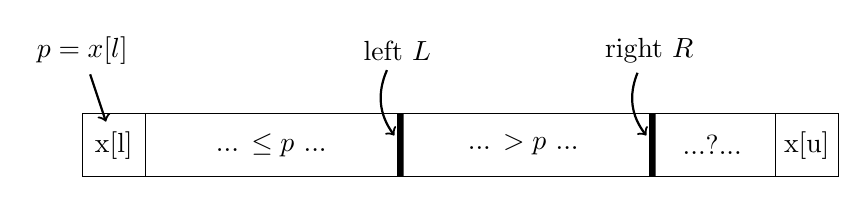
\begin{tikzpicture}[scale=0.8]
      \draw (0, 0) rectangle (1, 1) node (xl) [pos=.5] {x[l]}
            (1, 0) rectangle (5, 1) node (leq) [pos=.5] {... $\leq p$ ...}
            (5, 0) rectangle (9, 1) node (ge) [pos=.5] {... $> p$ ...}
            (9, 0) rectangle (11, 1) node (rest) [pos=.5] {...?...}
            (11, 0) rectangle (12, 1) node (xu) [pos=.5] {x[u]};
      \fill [black] (5, 0) rectangle (5.1, 1) node (leftbar) [pos=.5] {}
                    (9, 0) rectangle (9.1, 1) node (rightbar) [pos=.5] {};
      \draw (0, 2) node (pivot) {$p = x[l]$}
            (5, 2) node (left) {left $L$}
            (9, 2) node (right) {right $R$};
      \draw[thick, ->] (pivot) edge (xl)
                       (left) edge [bend right] (leftbar)
                       (right) edge [bend right] (rightbar);
      \end{tikzpicture}} \\
   \subcaptionbox{Initialize}{
      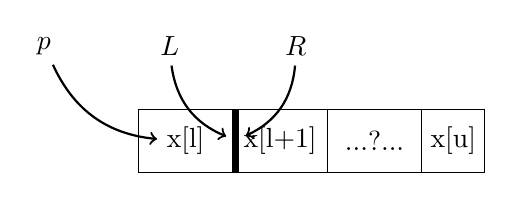
\begin{tikzpicture}[scale=0.8]
      \draw (-0.5, 0) rectangle (1, 1) node (xl) [pos=.5] {x[l]}
            (1, 0) rectangle (2.5, 1) node (xl1) [pos=.5] {x[l+1]}
            (2.5, 0) rectangle (4, 1) node (rest) [pos=.5] (ai) {...?...}
            (4, 0) rectangle (5, 1) node (xu) [pos=.5] {x[u]};
      \fill [black] (1, 0) rectangle (1.1, 1) node (leftbar) [pos=.5] {};
      \draw (-2, 2) node (pivot) {$p$}
            (0, 2) node (left) {$L$}
            (2, 2) node (right) {$R$};
      \draw[thick, ->] (pivot) edge [bend right] (xl)
                       (left) edge [bend right] (leftbar)
                       (right) edge [bend left] (leftbar);
      \end{tikzpicture}} \\
   \subcaptionbox{Terminate}{
      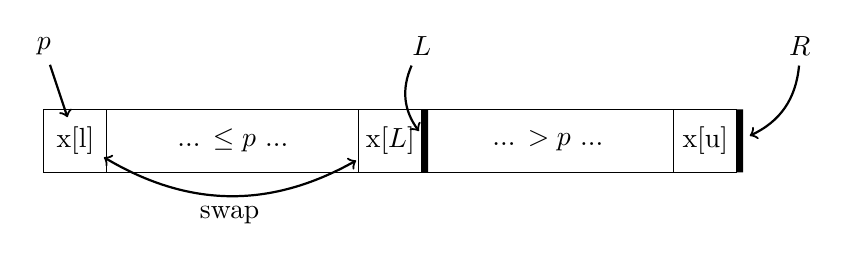
\begin{tikzpicture}[scale=0.8]
      \draw (0, 0) rectangle (1, 1) node (xl) [pos=.5] {x[l]}
            (1, 0) rectangle (5, 1) node (leq) [pos=.5] {... $\leq p$ ...}
            (5, 0) rectangle (6, 1) node (xleft) [pos=.5] {x[$L$] }
            (6, 0) rectangle (10, 1) node (ge) [pos=.5] {... $> p$ ...}
            (10, 0) rectangle (11, 1) node (xu) [pos=.5] {x[u]};
      \fill [black] (6, 0) rectangle (6.1, 1) node (leftbar) [pos=.5] {}
                    (11, 0) rectangle (11.1, 1) node (rightbar) [pos=.5] {};
      \draw (0, 2) node (pivot) {$p$}
            (6, 2) node (left) {$L$}
            (12, 2) node (right) {$R$};
      \draw[thick, ->] (pivot) edge (xl)
                       (left) edge [bend right] (leftbar)
                       (right) edge [bend left] (rightbar);
      \draw[thick, <->] (xl) edge [bend right] node [below] {swap} (xleft);
      \end{tikzpicture}} \\
   \caption{In-place partition, pivot $p = x[l]$}
   \label{fig:partition-1-way}
\end{figure}

\begin{itemize}
\item The pivot is the left element $p = x[l]$. It moves to the final position after partition;
\item A section of elements $\leq p$, extend right to $L$;
\item A section of elements $> p$, extend right to $R$. The elements between $L$ and $R$ $> p$;
\item Elements after $R$ haven't been partitioned (may $>, =, <$ p).
\end{itemize}

When partition starts, $L$ points to $p$, $R$ points to the next, as shown in figure \ref{fig:partition-1-way} (b). We advance $R$ to right till reach to the array boundary. Every time, we compare $x[R]$ and $p$. If $x[R] > p$, it should be between $L$ and $R$, we move $R$ forward; otherwise if $X[R] \leq p$, it should be on the left of $L$. We advance $L$ a step, then swap $x[L] \leftrightarrow x[R]$. When $R$ passes the last element, the partition ends. Elements $> p$ move to the right of $L$, while others on the left side. We need move $p$ to the position between the two parts. To do that, we swap $p \leftrightarrow x[L]$, as shown in \ref{fig:partition-1-way} (c). $L$ finally points to $p$, partitioned the array in two parts. We return $L + 1$ as the result, that points to the first element $> p$. Let the array be $A$, the lower, upper boundary be $l, u$. The in-place partition is defined below:

\begin{algorithmic}[1]
\Function{Partition}{A, l, u}
  \State $p \gets A[l]$  \Comment{pivot}
  \State $L \gets l$ \Comment{left}
  \For{$R$ in $[l+1, u]$} \Comment{iterate right}
    \If{$p \geq A[R]$}
      \State $L \gets L + 1$
      \State \textproc{Exchange} $A[L] \leftrightarrow A[R]$
    \EndIf
  \EndFor
  \State \textproc{Exchange} $A[L] \leftrightarrow p$
  \State \Return $L + 1$ \Comment{partition position}
\EndFunction
\end{algorithmic}

Table \ref{tab:partition-steps} lists the steps to partition $[3, 2, 5, 4, 0, 1, 6, 7]$.

\begin{table}[htbp]
\centering
\begin{tabular}{|llllllll|l|}
\hline
\underline{3}(l)  & 2(r) & 5 & 4 & 0 & 1 & 6 & 7 & start, $p = 3$、$l = 1$、$r = 2$ \\
\underline{3} & 2(l)(r) & 5 & 4 & 0 & 1 & 6 & 7 & $2 < 3$, advance $l$($r=l$)\\
\underline{3} & 2(l) & 5(r) & 4 & 0 & 1 & 6 & 7 & $5 > 3$, move on \\
\underline{3} & 2(l) & 5 & 4(r) & 0 & 1 & 6 & 7 & $4 > 3$, move on \\
\underline{3} & 2(l) & 5 & 4 & 0(r) & 1 & 6 & 7 & $0 < 3$ \\
\underline{3} & 2 & 0(l) & 4 & 5(r) & 1 & 6 & 7 & advance $l$, swap with $r$ \\
\underline{3} & 2 & 0(l) & 4 & 5 & 1(r) & 6 & 7 & $1 < 3$ \\
\underline{3} & 2 & 0 & 1(l) & 5 & 4(r) & 6 & 7 & advance $l$, swap with $r$ \\
\underline{3} & 2 & 0 & 1(l) & 5 & 4 & 6(r) & 7 & $6 > 3$, move on \\
\underline{3} & 2 & 0 & 1(l) & 5 & 4 & 6 & 7(r) & $7 > 3$, move on \\
1 & 2 & 0 & 3 & 5(l+1) & 4 & 6 & 7 & terminate, swap $p$ and $l$ \\
\hline
\end{tabular}
\caption{Partition array} \label{tab:partition-steps}
\end{table}

With \textproc{Partition} defined, we implement quick sort as below:

\begin{algorithmic}[1]
\Procedure{Quick-Sort}{$A, l, u$}
  \If{$l < u$}
    \State $m \gets$ \Call{Partition}{$A, l, u$}
    \State \Call{Quick-Sort}{$A, l, m - 1$}
    \State \Call{Quick-Sort}{$A, m, u$}
  \EndIf
\EndProcedure
\end{algorithmic}

We pass the array and its boundaries, as \textproc{Quick-Sort}($A, 1, |A|$) to sort. When the array is empty or singleton, sort returns immediately.

\begin{Exercise}
\Question{Improve the basic quick sort definition when the list is singleton.}
\end{Exercise}

\subsection{Performance}
\index{Quick sort!Performance}

Quick sort performs well in most cases. We start from the best/worst cases. For the best case, we always halve the elements into two equal sized parts. As shown in figure \ref{fig:qsort-best}, there are total $O(\lg n)$ levels of recursions. At level one, we processes $n$ elements with one partition; at level two, we partition twice, each processes $n/2$ elements, taking total $2 O(n/2) = O(n)$ time; at level three, we partition four times, each process $n/4$ elements, taking total $O(n)$ time too, ..., at the last level, there are $n$ singleton segments, taking total $O(n)$ time. Sum all levels, the time is bound to $O(n \lg n)$.

\begin{figure}[htbp]
 \centering
 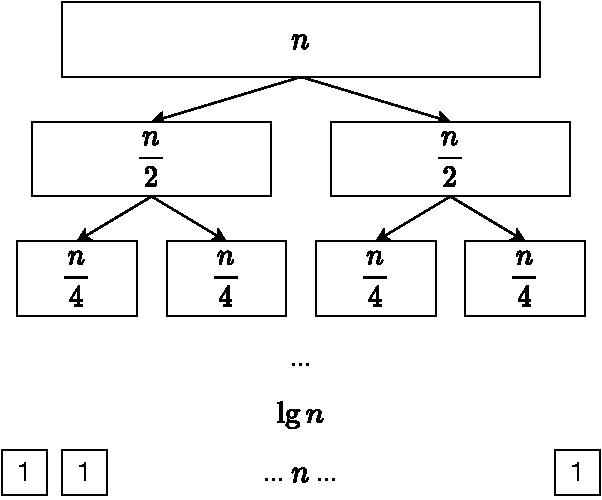
\includegraphics[scale=0.55]{img/qsort-best}
 \caption{The best case, halve every time.}
 \label{fig:qsort-best}
\end{figure}

For the worst case, the partition is totally unbalanced, one part is of $O(1)$ length, the other is $O(n)$. The level of recursions decays to $O(n)$. Model the partition as a tree. It's balanced binary tree in the best case, while it becomes a linked-list of $O(n)$ length in the worst case. Every branch node has an empty sub-tree. At each level, we process all elements, hence the total time is bound to $O(n^2)$. This is same as insertion sort, and selection sort. We can list several worst cases, for example, there are many duplicated elements, or the sequence is largely ordered, and so on. There isn't a method can avoid the worst case completely.

\subsubsection{Average case\texorpdfstring{$\bigstar$}{★}}
\index{Quick Sort!Average case}

Quick sort performs well in average. For example, even if every partition gives two parts of 1:9, the performance still achieves $O(n \lg n)$\cite{CLRS}. We give two method to evaluate the performance. The first one is based on the fact, that the performance is proportion to the number of comparisons. In selection sort, every two elements are compared, while in quick sort, we save many comparisons. When partition sequence $[a_1, a_2, a_3, ..., a_n]$ with $a_1$ as the pivot, we obtain two sub sequences $A = [x_1, x_2, ..., x_k]$ and $B = [y_1, y_2, ..., y_{n-k-1}]$. After that, none element in $A$ will compare with any one in $B$. Let the sorted result be $[a_1, a_2, ..., a_n]$, if $a_i < a_j$, we do not compare them if and only if there is some element $a_k$, where $a_i < a_k < a_j$, is picked as the pivot before either $a_i$ or $a_j$ being the pivot. In other word, the only chance that we compare $a_i$ and $a_j$ is either $a_i$ or $a_j$ is chosen as the pivot before any other elements in $a_{i+1} < a_{i+2} < ... < a_{j-1}$ being the pivot. Let $P(i, j)$ be the probability that we compare $a_i$ and $a_j$. We have:

\be
P(i, j) = \frac{2}{j - i + 1}
\ee

The total number of comparisons is:

\be
C(n) = \sum_{i=1}^{n-1}\sum_{j=i+1}^{n} P(i, j)
\ee

If we compare $a_i$ and $a_j$, we won't compare $a_j$ and $a_i$ again, and we never compare $a_i$ with itself. The upper bound of $i$ is $n-1$, and the lower bound of $j$ is $i+1$. Substitute the probability:

\be
\begin{array}{rl}
C(n) & = \displaystyle \sum_{i=1}^{n-1}\sum_{j = i+1}^{n} \frac{2}{j - i + 1} \\
     & = \displaystyle \sum_{i=1}^{n-1}\sum_{k=1}^{n-i} \frac{2}{k+1} \\
\end{array}
\ee

Use the result of harmonic series\cite{wiki-harmonic}.

\[
H_n = 1 + \frac{1}{2} + \frac{1}{3} + .... = \ln n + \gamma + \epsilon_n
\]

\be
C(n) = \sum_{i=1}^{n-1} O(\lg n) = O(n \lg n)
\ee

The other method uses the recursion. Let the length of the sequence be $n$, we partition it into two parts of length $i$ and $n-i-1$. The partition takes $cn$ time because it compares every element with the pivot. The total time is:

\be
T(n) = T(i) + T(n-i-1) + c n
\ee

Where $T(n)$ is the time to sort $n$ elements. $i$ equally distributes across $0, 1, ..., n-1$. Taking math expectation:

\be
\renewcommand*{\arraystretch}{1.5}
\begin{array}{rl}
T(n) & = E(T(i)) + E(T(n-i-1)) + c n \\
     & = \displaystyle \frac{1}{n} \sum_{i=0}^{n-1}T(i) + \frac{1}{n} \sum_{i=0}^{n-1}T(n-i-1) + cn \\
     & = \displaystyle \frac{1}{n} \sum_{i=0}^{n-1}T(i) + \frac{1}{n} \sum_{j=0}^{n-1}T(j) + cn \\
     & = \displaystyle \frac{2}{n} \sum_{i=0}^{b-1}T(i) + cn
\end{array}
\ee

Multiply $n$ to both sides:

\be
n T(n) = 2 \sum_{i=0}^{n-1} T(i) + c n^2
\label{eq:ntn}
\ee

Substitute $n$ to $n-1$:

\be
(n-1) T(n-1) = 2 \sum_{i=0}^{n-2} T(i) + c (n-1)^2
\label{eq:n1tn1}
\ee

Take (\ref{eq:ntn}) - (\ref{eq:n1tn1}), cancel all $T(i)$ for $0 \leq i < n-1$.

\be
n T(n) = (n + 1) T(n-1) + 2cn - c
\ee

Drop the constant $c$, we obtain:

\be
\frac{T(n)}{n+1} = \frac{T(n-1)}{n} + \frac{2c}{n+1}
\ee

Assign $n$ to $n-1$, $n-2$, ..., to give $n-1$ equations.

\[
\frac{T(n-1)}{n} = \frac{T(n-2)}{n-1} + \frac{2c}{n}
\]

\[
\frac{T(n-2)}{n-1} = \frac{T(n-3)}{n-2} + \frac{2c}{n-1}
\]

\[
...
\]

\[
\frac{T(2)}{3} = \frac{T(1)}{2} + \frac{2c}{3}
\]

Sum up and cancel the same components on both sides, we get a function of $n$.

\be
\frac{T(n)}{n+1} = \frac{T(1)}{2} + 2c \sum_{k=3}^{n+1} \frac{1}{k}
\ee

Use the result of the harmonic series:

\be
O(\frac{T(n)}{n+1}) = O(\frac{T(1)}{2} + 2c \ln n + \gamma + \epsilon_n) = O(\lg n)
\ee

Therefore:

\be
O(T(n)) = O(n \lg n)
\ee

\subsection{Improvement}
\index{Quick sort!Improvement} \index{Quick sort!Ternary partition}

The \textproc{Partition} procedure doesn't perform well when there are many duplicated elements. Consider the extreme case that all $n$ elements are equal $[x, x, ..., x]$:

\begin{enumerate}
\item From the quick sort definition: pick any element as the pivot, hence $p = x$, partition into two sub-sequences. One is $[x, x, ..., x]$ of length $n - 1$, the other is empty. Next recursively sort the $n-1$ elements, the total time decays to $O(n^2)$.
\item Modify the partition with $< x$ and $> x$. The result are two empty sub-sequences, and $n$ elements equal to $x$. The recursion on empty sequence terminates immediately. The result is $[\ ] \doubleplus [x, x, ..., x] \doubleplus [\ ]$. The performance is $O(n)$.
\end{enumerate}

We improve from {\em binary} partition to {\em ternary} partition to handle duplicated elements:

\be
\begin{array}{rcl}
sort\ [\ ] & = & [\ ] \\
sort\ (x \cons xs) & = & sort\ S \doubleplus sort\ E \doubleplus sort\ G
\end{array}
\ee

Where:

\[
\begin{cases}
S = [ y | y \in xs, y < x ] \\
E = [ y | y \in xs, y = x ] \\
G = [ y | y \in xs, y > x ] \\
\end{cases}
\]

To concatenate three lists in linear time, we can use an accumulator: $qsort = sort\ [\ ]$, where:

\be
\begin{array}{rcl}
sort\ A\ [\ ] & = & A \\
sort\ A\ (x \cons xs) & = & sort\ (E \doubleplus sort\ A\ G)\ S \\
\end{array}
\ee

We partition the list in three parts: $S, E, G$, where $E$ contains elements of same value, hence sorted. We first sort $G$ with accumulator $A$, append the result to $E$ as the new accumulator, and use it to sort $S$. We also improve the partition with accumulator:

\be
\begin{array}{rcl}
part\ S\ E\ G\ x\ [\ ] & = & (S, E, G) \\
part\ S\ E\ G\ x\ (y \cons ys) & = & \begin{cases}
  y < x: & (y \cons S, E, G) \\
  y = x: & (S, y \cons E, G) \\
  y > x: & (S, E, y \cons G) \\
  \end{cases} \\
\end{array}
\ee

Richard Bird developed another improvement\cite{fp-pearls}, instead concatenate the
recursive sort results, put them in a list and concatenate finally:

\begin{Haskell}
sort :: (Ord a) => [a] -> [a]
sort = concat . (pass [])

pass xss [] = xss
pass xss (x:xs) = step xs [] [x] [] xss where
    step [] as bs cs xss = pass (bs : pass xss cs) as
    step (x':xs') as bs cs xss | x' <  x = step xs' (x':as) bs cs xss
                               | x' == x = step xs' as (x':bs) cs xss
                               | x' >  x = step xs' as bs (x':cs) xss
\end{Haskell}

\index{Quick Sort!2-way partition}
Robert Sedgewick developed two-way partition method\cite{qsort-impl}\cite{Bentley}. Use two pointers $i, j$ from left and right boundaries. Pick the first element as the pivot $p$. Advance $i$ to right till an element $\geq p$; while (in parallel) move $j$ to left till an element $\leq p$. At this time, all elements left to $i$ are less than the pivot ($< p$), while those right to $j$ are greater than the pivot ($> p$). $i$ points to one that $\geq p$, and $j$ points to one that $\leq p$, as shown in figure \ref{fig:partition-2-way} (a). To move all elements $\leq p$ to left, and the remaining to right, we exchange $x[i] \leftrightarrow x[j]$, then continue scan. We repeat this till $i$ and $j$ meet. At any time, we keep the invariant: All elements left to $i$ (include $i$) are $\leq p$; while all right to $j$ (include $j$) are $\geq p$. The elements between $i$ and $j$ are yet to scan, as shown in figure \ref{fig:partition-2-way} (b).

\begin{figure}[htbp]
   \centering
   \subcaptionbox{When $i$ and $j$ stop}{
      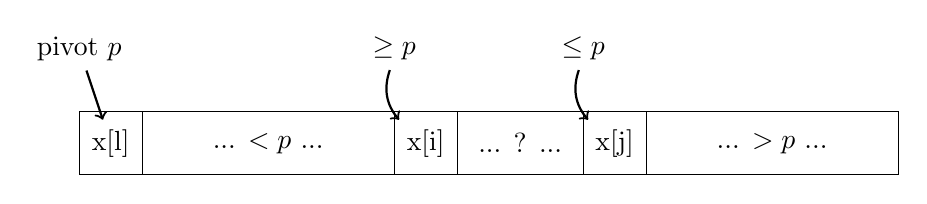
\begin{tikzpicture}[scale=0.8]
      \draw (0, 0) rectangle (1, 1) node (xl) [pos=.5] {x[l]}
            (1, 0) rectangle (5, 1) node (leq) [pos=.5] {... $< p$ ...}
            (5, 0) rectangle (6, 1) node (xi) [pos=.5] {x[i]}
            (6, 0) rectangle (8, 1) node (rest) [pos=.5] {... ? ...}
            (8, 0) rectangle (9, 1) node (xj) [pos=.5] {x[j]}
            (9, 0) rectangle (13, 1) node (ge) [pos=.5] {... $> p$ ...};
      \draw (0, 2) node (pivot) {pivot $p$}
            (5, 2) node (left) {$\geq p$}
            (8, 2) node (right) {$\leq p$};
      \draw[thick, ->] (pivot) edge (xl)
                       (left) edge [bend right] (xi)
                       (right) edge [bend right] (xj);
      \end{tikzpicture}} \\
   \subcaptionbox{Partition invariant}{
      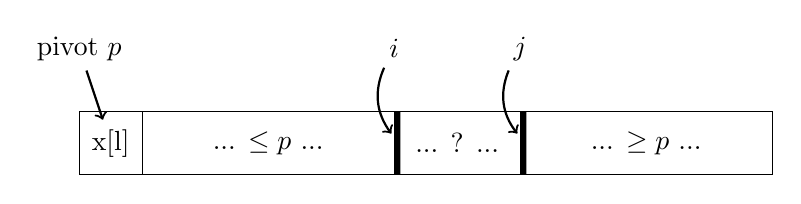
\begin{tikzpicture}[scale=0.8]
      \draw (0, 0) rectangle (1, 1) node (xl) [pos=.5] {x[l]}
            (1, 0) rectangle (5, 1) node (leq) [pos=.5] {... $\leq p$ ...}
            (5, 0) rectangle (7, 1) node (rest) [pos=.5] {... ? ...}
            (7, 0) rectangle (11, 1) node (ge) [pos=.5] {... $\geq p$ ...};
      \fill [black] (5, 0) rectangle (5.1, 1) node (ibar) [pos=.5] {}
                    (7, 0) rectangle (7.1, 1) node (jbar) [pos=.5] {};
      \draw (0, 2) node (pivot) {pivot $p$}
            (5, 2) node (i) {$i$}
            (7, 2) node (j) {$j$};
      \draw[thick, ->] (pivot) edge (xl)
                       (i) edge [bend right] (ibar)
                       (j) edge [bend right] (jbar);
      \end{tikzpicture}} \\
   \caption{2-way scan}
   \label{fig:partition-2-way}
\end{figure}

When $i$ meets $j$, we need an extra exchange, swap the pivot $p$ to position $j$. Then recursive sort sub-array $A[l ... j)$ and $A[i ... u)$.

\begin{algorithmic}[1]
\Procedure{Sort}{$A, l, u$} \Comment{sort range $[l, u)$}
  \If{$u - l > 1$} \Comment{At least 2 elements}
    \State $i \gets l$, $j \gets u$
    \State $pivot \gets A[l]$
    \Loop
      \Repeat
        \State $i \gets i + 1$
      \Until{$A[i] \geq pivot$} \Comment{Ignore $i \geq u$}
      \Repeat
        \State $j \gets j - 1$
      \Until{$A[j] \leq pivot$} \Comment{Ignore $j < l$}
      \If{$j < i$}
        \State break
      \EndIf
      \State \textproc{Exchange} $A[i] \leftrightarrow A[j]$
    \EndLoop
    \State \textproc{Exchange} $A[l] \leftrightarrow A[j]$ \Comment{Move the pivot}
    \State \Call{Sort}{$A, l, j$}
    \State \Call{Sort}{$A, i, u$}
  \EndIf
\EndProcedure
\end{algorithmic}

\index{Quick Sort!3-way partition}
Consider the special case that all elements are equal, the array is partitioned into two same parts with $\dfrac{n}{2}$ swaps. Because of the balanced partition, the performance is $O(n \lg n)$. It takes less swaps than the one pass scan method, since it skips the elements on the right side of the pivot. We can combine 2-way scan and ternary partition. Only recursively sort the elements different with the pivot. Jon Bentley and Douglas McIlroy developed a method as shown in figure \ref{fig:partition-3-way} (a), that store the elements equal to the pivot on both sides\cite{3-way-part}\cite{opt-qs}.

\begin{figure}[htbp]
   \centering
   \subcaptionbox{Ternary partition invariant.}{
      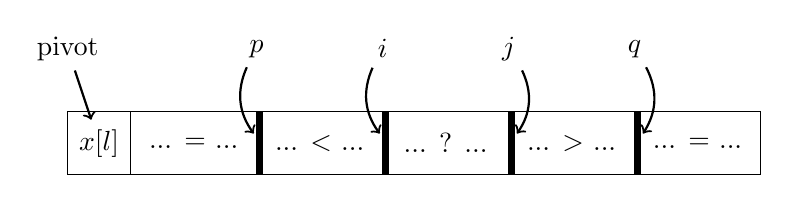
\begin{tikzpicture}[scale=0.8]
      \draw (0, 0) rectangle (1, 1) node (xl) [pos=.5] {$x[l]$}
            (1, 0) rectangle (3, 1) node [pos=.5] {... $=$ ...}
            (3, 0) rectangle (5, 1) node [pos=.5] {... $<$ ...}
            (5, 0) rectangle (7, 1) node [pos=.5] {... ? ...}
            (7, 0) rectangle (9, 1) node [pos=.5] {... $>$ ...}
            (9, 0) rectangle (11, 1) node [pos=.5] {... $=$ ...};
      \fill [black] (3, 0) rectangle (3.1, 1) node (pbar) [pos=.5] {}
                    (5, 0) rectangle (5.1, 1) node (ibar) [pos=.5] {}
                    (7, 0) rectangle (7.1, 1) node (jbar) [pos=.5] {}
                    (9, 0) rectangle (9.1, 1) node (qbar) [pos=.5] {};
      \draw (0, 2) node (pivot) {pivot}
            (3, 2) node (p) {$p$}
            (5, 2) node (i) {$i$}
            (7, 2) node (j) {$j$}
            (9, 2) node (q) {$q$};
      \draw[thick, ->] (pivot) edge (xl)
                       (p) edge [bend right] (pbar)
                       (i) edge [bend right] (ibar)
                       (j) edge [bend left] (jbar)
                       (q) edge [bend left] (qbar);
      \end{tikzpicture}} \\
   \subcaptionbox{Swap the elements $= p$ to the middle.}{\hspace{0.1\textwidth}
      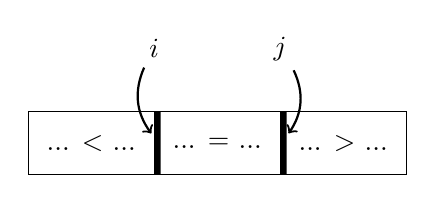
\begin{tikzpicture}[scale=0.8]
      \draw (0, 0) rectangle (2, 1) node [pos=.5] {... $<$ ...}
            (2, 0) rectangle (4, 1) node [pos=.5] {... $=$ ...}
            (4, 0) rectangle (6, 1) node [pos=.5] {... $>$ ...};
      \fill [black] (2, 0) rectangle (2.1, 1) node (ibar) [pos=.5] {}
                    (4, 0) rectangle (4.1, 1) node (jbar) [pos=.5] {};
      \draw (2, 2) node (i) {$i$}
            (4, 2) node (j) {$j$};
      \draw[thick, ->] (i) edge [bend right] (ibar)
                       (j) edge [bend left] (jbar);
      \end{tikzpicture}
      \hspace{0.1\textwidth}}
   \caption{Ternary partition}
   \label{fig:partition-3-way}
\end{figure}

We scan from two sides, pause when $i$ reach an element $\geq$ the pivot, and $j$ reach one $\leq$ the pivot. If $i$ doesn't meet or pass $j$, we exchange $A[i] \leftrightarrow A[j]$, then check if $A[i]$ or $A[j]$ equals to the pivot. If yes, we exchange $A[i] \leftrightarrow A[p]$ or $A[j] \leftrightarrow A[q]$ respectively. Finally, we swap all the elements equal to the pivot to the middle. This step do nothing if all elements are unique. The partition result is shown as \ref{fig:partition-3-way} (b). We next only recursively sort the elements not equal to the pivot.

\begin{algorithmic}[1]
\Procedure{Sort}{$A, l, u$}
  \If{$u - l > 1$}
    \State $i \gets l$, $j \gets u$
    \State $p \gets l$, $q \gets u$ \Comment{point to the boundaries of duplicated elements}
    \State $pivot \gets A[l]$
    \Loop
      \Repeat
        \State $i \gets i + 1$
      \Until{$A[i] \geq pivot$} \Comment{Ignore $i \geq u$ case}
      \Repeat
        \State $j \gets j - 1$
      \Until{$A[j] \leq pivot$} \Comment{Ignore $j < l$ case}
      \If{$j \leq i$}
        \State break
      \EndIf
      \State \textproc{Exchange} $A[i] \leftrightarrow A[j]$
      \If{$A[i] = pivot$} \Comment{duplicated element}
        \State $p \gets p + 1$
        \State \textproc{Exchange} $A[p] \leftrightarrow A[i]$
      \EndIf
      \If{$A[j] = pivot$}
        \State $q \gets q - 1$
        \State \textproc{Exchange} $A[q] \leftrightarrow A[j]$
      \EndIf
    \EndLoop
    \If{$i = j$ and $A[i] = pivot$}
      \State $j \gets j - 1$, $i \gets i + 1$
    \EndIf
    \For{$k$ from $l$ to $p$} \Comment{Swap the duplicated elements to the middle}
      \State \textproc{Exchange} $A[k] \leftrightarrow A[j]$
      \State $j \gets j - 1$
    \EndFor
    \For{$k$ from $u-1$ down-to $q$}
      \State \textproc{Exchange} $A[k] \leftrightarrow A[i]$
      \State $i \gets i + 1$
    \EndFor
    \State \Call{Sort}{$A, l, j + 1$}
    \State \Call{Sort}{$A, i, u$}
  \EndIf
\EndProcedure
\end{algorithmic}

It becomes complex when combine 2-way scan and ternary partition. We can change the one pass scan to ternary partition directly. Pick the first element as the pivot, as shown in figure \ref{fig:partition-3-way-lumoto}. At any time, the left part contains elements $< p$; the next part contains those $= p$; and the right part contains those $> p$. The boundaries are $i, k, j$. Elements between $[k, j)$ are yet to be partitioned. We scan from left to right. When start, the part $< p$ is empty; the part $= p$ has an element; $i$ points to the lower boundary, $k$ points to the next. The part $> p$ is empty too, $j$ points to the upper boundary.

\begin{figure}[htbp]
   \centering
      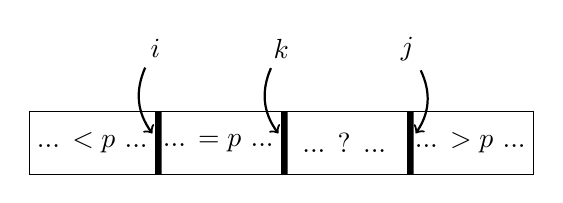
\begin{tikzpicture}[scale=0.8]
      \draw (0, 0) rectangle (2, 1) node [pos=.5] {... $< p$ ...}
            (2, 0) rectangle (4, 1) node [pos=.5] {... $= p$ ...}
            (4, 0) rectangle (6, 1) node [pos=.5] {... ? ...}
            (6, 0) rectangle (8, 1) node [pos=.5] {... $> p$ ...};
      \fill [black] (2, 0) rectangle (2.1, 1) node (ibar) [pos=.5] {}
                    (4, 0) rectangle (4.1, 1) node (kbar) [pos=.5] {}
                    (6, 0) rectangle (6.1, 1) node (jbar) [pos=.5] {};
      \draw (2, 2) node (i) {$i$}
            (4, 2) node (k) {$k$}
            (6, 2) node (j) {$j$};
      \draw[thick, ->] (i) edge [bend right] (ibar)
                       (k) edge [bend right] (kbar)
                       (j) edge [bend left] (jbar);
      \end{tikzpicture}
   \caption{1 way scan ternary partition}
   \label{fig:partition-3-way-lomuto}
\end{figure}

We iterate on $k$, if $A[k] = p$, then move $k$ to the next; if $A[k] > p$, then exchange $A[k] \leftrightarrow A[j-1]$, the range of elements that $> p$ increases by one. Its boundary $j$ moves to left a step. Because we don't know if the element moved to $k$ is still $> p$, we compare again and repeat. Otherwise if $A[k] < p$, we exchange $A[k] \leftrightarrow A[i]$, where $A[i]$ is the first element that $= p$. The partition terminates when $k$ meets $j$.

\begin{algorithmic}[1]
\Procedure{Sort}{$A, l, u$}
  \If{$u - l > 1$}
    \State $i \gets l$, $j \gets u$, $k \gets l + 1$
    \State $pivot \gets A[i]$
    \While{$k < j$}
      \While{$pivot < A[k]$}
        \State $j \gets j - 1$
        \State \textproc{Exchange} $A[k] \leftrightarrow A[j]$
      \EndWhile
      \If{$A[k] < pivot$}
        \State \textproc{Exchange} $A[k] \leftrightarrow A[i]$
        \State $i \gets i + 1$
      \EndIf
      \State $k \gets k + 1$
    \EndWhile
    \State \Call{Sort}{$A, l, i$}
    \State \Call{Sort}{$A, j, u$}
  \EndIf
\EndProcedure
\end{algorithmic}

Compare with the ternary partition through 2-way scan, this implementation is less complex but need more swaps.

\subsubsection{Worst cases}

Although ternary partition handles duplicated elements well, there are the worst cases. For example, when most elements are ordered (ascending or descending), the partition is unbalanced. Figure \ref{fig:worst-cases-1} gives two of the worst cases: $[x_1 < x_2 < ... < x_n]$ and $[y_1 > y_2 > ... > y_n]$. It's easy to give more, for example: $[x_m, x_{m-1}, ..., x_2, x_1, x_{m+1}, x_{m+2}, ... x_n]$, where $[ x_1 < x_2 < ... < x_n]$, and $[x_n, x_1, x_{n-1}, x_2, ... ]$ as shown in figure \ref{fig:worst-cases-2}.

\begin{figure}[htbp]
   \centering
   \subcaptionbox{Partition tree of $[x_1 < x_2 < ... < x_n]$, the sub-trees of $\leq p$ are empty.}{\hspace{.3\textwidth} 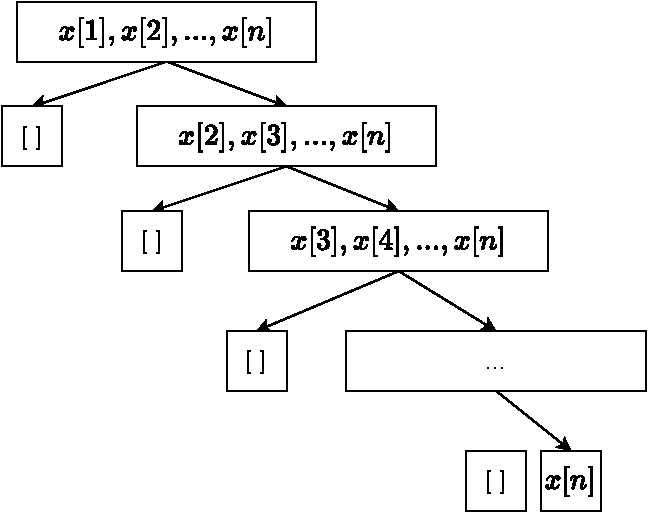
\includegraphics[scale=0.5]{img/unbalanced} \hspace{.3\textwidth}} \\
   \subcaptionbox{Partition tree of $[y_1 > y_2 > ... > y_n]$, the sub-trees of $\geq p$ are empty.}{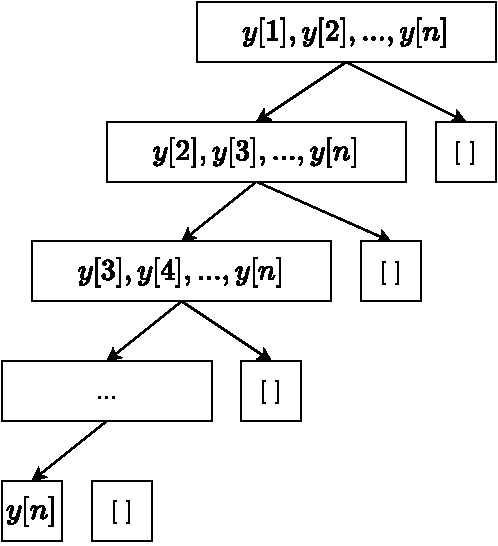
\includegraphics[scale=0.5]{img/unbalanced-2}} \\
   \caption{The worst cases - 1.}
   \label{fig:worst-cases-1}
\end{figure}

\begin{figure}[htbp]
   \centering
   \subcaptionbox{Unbalanced partitions except for the first time.}{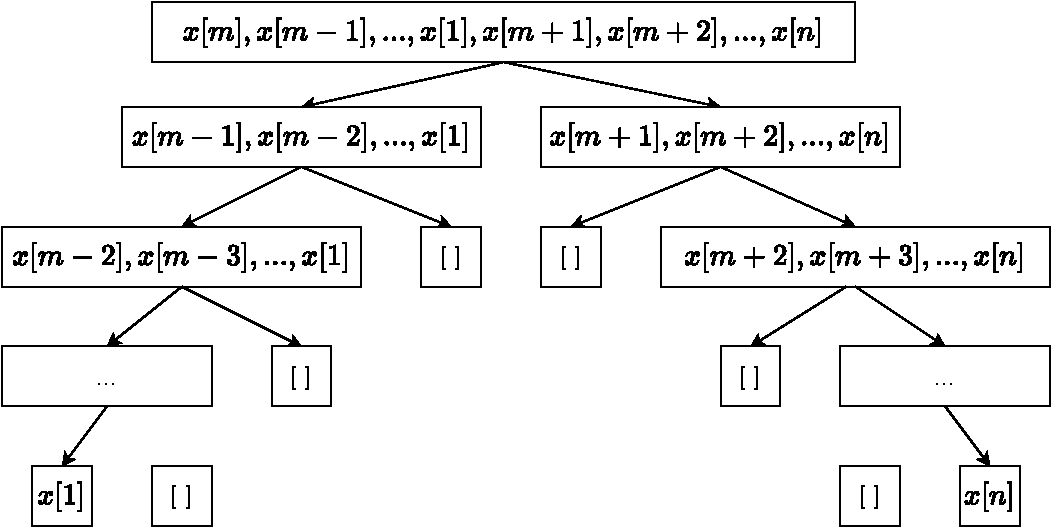
\includegraphics[scale=0.4]{img/unbalanced-3}} \\
   \subcaptionbox{A zig-zag partition tree.}{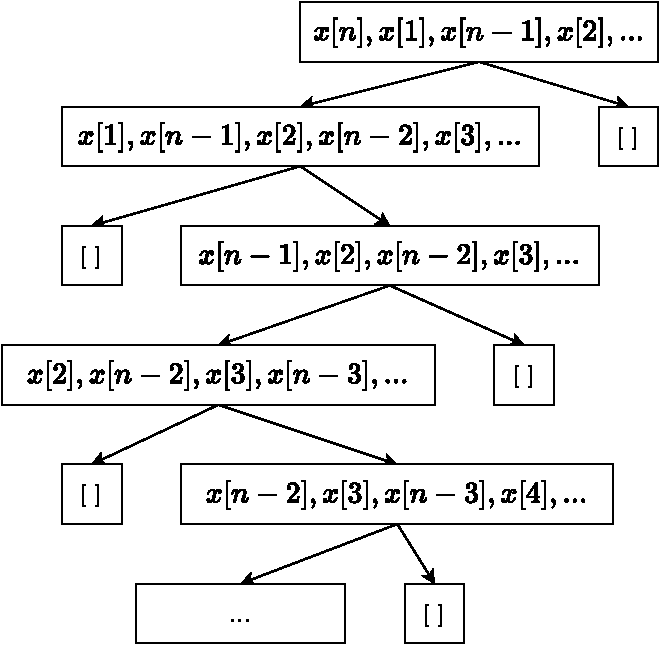
\includegraphics[scale=0.5]{img/unbalanced-zigzag}} \\
   \caption{The worst cases - 2.}
   \label{fig:worst-cases-2}
\end{figure}

In these worst cases, the partition is unbalanced when choose the first element as the pivot. Robert Sedgwick improved the pivot selection\cite{qsort-impl}: Instead pick a fixed position, sample several elements to avoid bad pivot. We sample the first, the middle, and the last, pick the median as the pivot. We can either compare every two (total 3 times)\cite{3-way-part}, or swap the least one to head, swap the greatest one end, and move the median to the middle.

\begin{algorithmic}[1]
\Procedure{Sort}{$A, l, u$}
  \If{$u - l > 1$}
    \State $m \gets \lfloor \dfrac{l + u}{2} \rfloor$ \Comment{or $l + \dfrac{u - l}{2}$ to void overflow}
    \If{$A[m] < A[l]$} \Comment{Ensure $A[l] \leq A[m]$}
      \State \textproc{Exchange} $A[l] \leftrightarrow A[m]$
    \EndIf
    \If{$A[u-1] < A[l]$} \Comment{Ensure $A[l] \leq A[u-1]$}
      \State \textproc{Exchange} $A[l] \leftrightarrow A[u-1]$
    \EndIf
    \If{$A[u-1] < A[m]$} \Comment{Ensure $A[m] \leq A[u-1]$}
      \State \textproc{Exchange} $A[m] \leftrightarrow A[u-1]$
    \EndIf
    \State \textproc{Exchange} $A[l] \leftrightarrow A[m]$
    \State $(i, j) \gets $ \Call{Partition}{$A, l, u$}
    \State \Call{Sort}{$A, l, i$}
    \State \Call{Sort}{$A, j, u$}
  \EndIf
\EndProcedure
\end{algorithmic}

This implementation handles the above four worst cases well. We call it `median of three'. Alternatively, we can randomly pick pivot:

\begin{algorithmic}[1]
\Procedure{Sort}{$A, l, u$}
  \If{$u - l > 1$}
    \State \textproc{Exchange} $A[l] \leftrightarrow A[$ \Call{Random}{$l, u$} $]$
    \State $(i, j) \gets $ \Call{Partition}{$A, l, u$}
    \State \Call{Sort}{$A, l, i$}
    \State \Call{Sort}{$A, j, u$}
  \EndIf
\EndProcedure
\end{algorithmic}

Where \textproc{Random}($l, u$) returns integer $l \leq i < u$ randomly. We swap $A[i]$ with the first element as the pivot. This method is called {\em random quick sort} \cite{CLRS}. Theoretically, neither `median of three' nor random quick sort can avoid the worst case completely. If the sequence is random, it's same to choose any one as the pivot. Nonetheless, these improvements are widely used in engineering practice.

There are other improvements besides partition. Sedgewick found quick sort had overhead when the list is short, while insert sort performed better\cite{Bentley}\cite{3-way-part}. Sedgewick, Bentley and McIlroy evaluated varies thresholds, as `cut-off'. When the elements are less than the `cut-off', then switch to insert sort.

\begin{algorithmic}[1]
\Procedure{Sort}{$A, l, u$}
  \If{$u - l > $ \textproc{Cut-Off}}
    \State \Call{Quick-Sort}{$A, l, u$}
  \Else
    \State \Call{Insertion-Sort}{$A, l, u$}
  \EndIf
\EndProcedure
\end{algorithmic}

\subsection{quick sort and tree sort}

The `true quick sort' is the combination of multiple engineering improvements, falls back to insert sort for small sequence, in-place swaps, choose the pivot as the `median of three', 2-way scan, and ternary partition. Some people think the basic recursive definition is essentially tree sort. Richard Bird derived quick sort from binary tree sort by deforestation\cite{algo-fp}. Define \textit{unfold} that converts a list to binary search tree:

\be
\begin{array}{rcl}
\textit{unfold}\ [\ ] & = & \nil \\
\textit{unfold}\ (x \cons xs) & = & (\textit{unfold}\ [a | a \in xs, a \leq x], x, \textit{unfold}\ [a | a \in xs, a > x]) \\
\end{array}
\ee

Compare with the binary tree insert (see chapter 2), \textit{unfold} creates the tree differently. If the list is empty, the tree is empty; otherwise, use the first element $x$ as the key, then recursively build the left, right sub-trees. Where the left sub-tree has the elements $\leq x$; and the right tree has elements that $> x$. While to convert a binary search tree to ordered list, we define in-order traverse as:

\be
\begin{array}{rcl}
\textit{toList}\ \nil & = & [\ ] \\
\textit{toList}\ (l, k, r) & = & \textit{toList}\ l \doubleplus [k] \doubleplus \textit{toList}\ r \\
\end{array}
\ee

We define quick sort by composing the two functions:

\be
\textit{sort} = \textit{toList} \circ \textit{unfold}
\ee

We first build the binary search tree through \textit{unfold}, then pass it to \textit{toList} to generate the list, and discard the tree. When eliminate the intermediate tree (through {\em deforestation} by Burstle-Darlington's work\cite{slpj}), we obtain the quick sort.

\section{Merge sort}
\index{Merge Sort}

Quick sort performs well in most cases. However, there are the worst cases can't be completely avoided. Merge sort guarantees $O(n \lg n)$ performance in all cases. It supports both arrays and lists. Many programming environments provide merge sort as the standard sort tool\footnote{For example in the standard library of Haskell, Python, and Java.}. Merge sort takes divide and conquer approach. It always splits the sequence in half and half, recursively sort them and merge.

\be
\begin{array}{rcl}
sort\ [\ ] & = & [\ ] \\
sort\ [x] & = & [x] \\
sort\ xs & = & merge\ (sort\ as)\ (sort\ bs), \text{where}: (as, bs) = \textit{halve}\ xs
\end{array}
\ee

Where \textit{halve} splits the sequence, for array, we can cut at the middle: $\textit{splitAt}\ \lfloor \dfrac{|xs|}{2} \rfloor\ xs$. However, it takes linear time to move to the middle point of a list (see chapter 1):

\be
\textit{splitAt}\ n\ xs = \textit{shift}\ n\ [\ ]\ xs
\ee

Where:

\be
\begin{array}{rcl}
\textit{shift}\ 0\ as\ bs & = & (as, bs) \\
\textit{shift}\ n\ as\ (b \cons bs) & = & \textit{shift}\ (n - 1)\ (b \cons as)\ bs
\end{array}
\ee

Because \textit{halve} needn't keep the relative order among elements, we can simplify the implementation with odd-even split. There are same number of elements in odd and even positions, or they only differ by one. $\textit{halve} = \textit{split}\ [\ ]\ [\ ]$, where:

\be
\begin{array}{rcl}
\textit{split}\ as\ bs\ [\ ] & = & (as, bs) \\
\textit{split}\ as\ bs\ [x] & = & (x \cons as, bs) \\
\textit{split}\ as\ bs\ (x \cons y \cons xs) & = & \textit{split}\ (x \cons as)\ (y \cons bs)\ xs \\
\end{array}
\ee

We can further simplify it with folding, as in below example, we add $x$ to $a$ every time, then swap $as \leftrightarrow bs$:

\begin{Haskell}
halve = foldr f ([], []) where
  f x (as, bs) = (bs, x : as)
\end{Haskell}

\subsection{Merge}
\index{Merge Sort!Merge}

Merge is demonstrated as figure \ref{fig:merge}. Consider two groups of kids, already ordered from short to tall. They need pass a gate, one kid per time. We arrange the first kid from each group to compare, the shorter one pass the gate. Repeat this till a group pass the gate, then the remaining kids pass the gate one by one.

\begin{figure}[htbp]
 \centering
 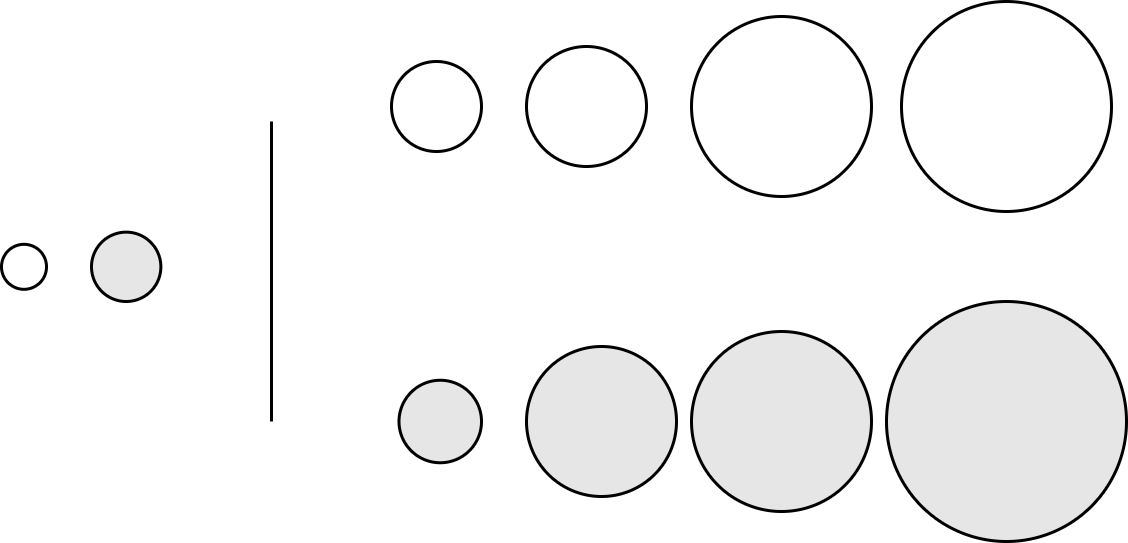
\includegraphics[scale=0.3]{img/merge2w}
 \caption{Merge}
 \label{fig:merge}
\end{figure}

\be
\begin{array}{rcl}
\textit{merge}\ [\ ]\ bs & = & bs \\
\textit{merge}\ as\ [\ ] & = & as \\
\textit{merge}\ (a \cons as)\ (b \cons bs) & = & \begin{cases}
  a < b: & a : \textit{merge}\ as\ (b \cons bs) \\
  \text{otherwise}: & b : \textit{merge}\ (a \cons as)\ bs
  \end{cases}
\end{array}
\ee

For array, we directly cut at the middle position, recursively sort two halves, then merge:

\begin{algorithmic}[1]
\Procedure{Sort}{$A$}
  \State $n \gets |A|$
  \If{$n > 1$}
    \State $m \gets \lfloor \dfrac{n}{2} \rfloor$
    \State $X \gets$ \Call{Copy-Array}{$A[1...m]$}
    \State $Y \gets$ \Call{Copy-Array}{$A[m+1...n]$}
    \State \Call{Sort}{$X$}
    \State \Call{Sort}{$Y$}
    \State \Call{Merge}{$A, X, Y$}
  \EndIf
\EndProcedure
\end{algorithmic}

We allocated additional space of the same size of $A$ because \textproc{Merge} is not in-pace. We repeatedly compare elements from $X$ and $Y$, pick the less one to $A$. When either sub-array finish, we add all the remaining to $A$.

\begin{algorithmic}[1]
\Procedure{Merge}{$A, X, Y$}
  \State $i \gets 1, j\gets 1, k\gets 1$
  \State $m \gets |X|, n \gets |Y|$
  \While{$i \leq m$ and $j \leq n$}
    \If{$X[i] < Y[j]$}
      \State $A[k] \gets X[i]$
      \State $i \gets i + 1$
    \Else
      \State $A[k] \gets Y[j]$
      \State $j \gets j + 1$
    \EndIf
    \State $k \gets k + 1$
  \EndWhile
  \While{$i \leq m$}
    \State $A[k] \gets X[i]$
    \State $k \gets k + 1$
    \State $i \gets i + 1$
  \EndWhile
  \While{$j \leq n$}
    \State $A[k] \gets Y[j]$
    \State $k \gets k + 1$
    \State $j \gets j + 1$
  \EndWhile
\EndProcedure
\end{algorithmic}

\subsection{Performance}
\index{Merge Sort!Performance}

Merge sort has two steps: partition and merge. We always halve the sequence. The partition tree is a balanced binary tree as shown in figure \ref{fig:qsort-best}. The height is $O(\lg n)$, so as the recursion depth. The merge happens at every level, compares elements one by one from each sorted sub-sequence. Hence merge takes linear time. For sequence of length $n$, let $T(n)$ be the merge sort time, we have below recursive breakdown:

\be
T(n) = T(\dfrac{n}{2}) + T(\dfrac{n}{2}) + c n = 2 T(\dfrac{n}{2}) + c n
\ee

The time consists of three parts: sort the first half, sort the second half, each takes $T(\dfrac{n}{2})$ time; and merge in $c n$ time, where $c$ is a constant. Solving this equation gives $O(n \lg n)$ result. The other performance factor is space. Varies implementation differ a lot. The basic merge sort allocates the space of the same size as the array in each recursion, copies elements and sorts, then release the space. When reach to the deepest recursion, consume the largest space of $O(n \lg n)$.

\subsubsection{Improvement}
\index{Merge Sort!Work area}

To simplify merge, we append $\infty$ to $X$ and $Y$\footnote{$-\infty$ for descending order}.

\begin{algorithmic}[1]
\Procedure{Merge}{$A, X, Y$}
  \State \Call{Append}{$X, \infty$}
  \State \Call{Append}{$Y, \infty$}
  \State $i \gets 1, j\gets 1, n \gets |A|$
  \For{$k \gets$ from 1 to $n$}
    \If{$X[i] < Y[j]$}
      \State $A[k] \gets X[i]$
      \State $i \gets i + 1$
    \Else
      \State $A[k] \gets Y[j]$
      \State $j \gets j + 1$
    \EndIf
  \EndFor
\EndProcedure
\end{algorithmic}

It's expensive to allocate/release space repeatedly\cite{Bentley}. We can pre-allocate a work area of the same size as $A$. Reuse it during recursive merge, and finally release it.

\begin{algorithmic}[1]
\Procedure{Sort}{A}
  \State $n \gets |A|$
  \State \textproc{Sort$'$}$(A$, \Call{Create-Array}{$n$}, $1, n)$
\EndProcedure
\Statex
\Procedure{Sort$'$}{$A, B, l, u$}
  \If{$u - l > 0$}
    \State $m \gets \lfloor \dfrac{l + u}{2} \rfloor$
    \State \Call{Sort$'$}{$A, B, l, m$}
    \State \Call{Sort$'$}{$A, B, m + 1, u$}
    \State \Call{Merge$'$}{$A, B, l, m, u$}
  \EndIf
\EndProcedure
\end{algorithmic}

We need update \textproc{Merge$'$} with the passed in work area:

\begin{algorithmic}[1]
\Procedure{Merge$'$}{$A, B, l, m, u$}
  \State $i \gets l, j \gets m + 1, k \gets l$
  \While{$i \leq m$ and $j \leq u$}
    \If{$A[i] < A[j]$}
      \State $B[k] \gets A[i]$
      \State $i \gets i + 1$
    \Else
      \State $B[k] \gets A[j]$
      \State $j \gets j + 1$
    \EndIf
    \State $k \gets k + 1$
  \EndWhile
  \While{$i \leq m$}
    \State $B[k] \gets A[i]$
    \State $k \gets k + 1$
    \State $i \gets i + 1$
  \EndWhile
  \While{$j \leq u$}
    \State $B[k] \gets A[j]$
    \State $k \gets k + 1$
    \State $j \gets j + 1$
  \EndWhile
  \For{$i \gets$ from $l$ to $u$} \Comment{copy back}
    \State $A[i] \gets B[i]$
  \EndFor
\EndProcedure
\end{algorithmic}

This implementation reduces the space from $O(n \lg n)$ to $O(n)$, improve performance 20\% to 25\% for 100,000 numeric elements.

\subsection{In-place merge sort}
\index{Merge Sort!In-place merge sort}

To avoid additional space, we consider how to reuse the array as the work area. As shown in figure \ref{fig:merge-in-place-naive}, sub-array $A$ and $B$ are sorted, when merge in-place, the part before $l$ are merged and ordered. If $A[l] < A[m]$, move $l$ to right a step; otherwise if $A[l] \geq A[m]$, we need move $A[m]$ to merge result before $l$. We need shift all elements between $l$ and $m$ (including $l$) to right a step.

\begin{figure}[htbp]
 \centering
      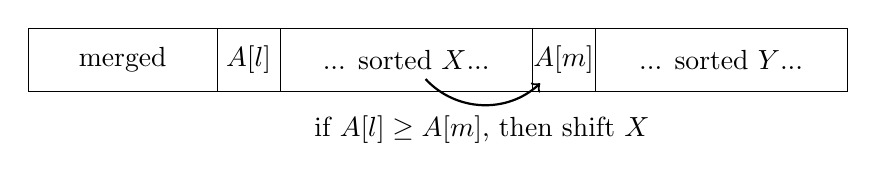
\begin{tikzpicture}[scale=0.8]
      \draw (0, 0) rectangle (3, 1) node [pos=.5] {merged}
            (3, 0) rectangle (4, 1) node [pos=.5] {$A[l]$}
            (4, 0) rectangle (8, 1) node (subA) [pos=.5] {... sorted $X$...}
            (8, 0) rectangle (9, 1) node (xsj) [pos=.5] {$A[m]$}
            (9, 0) rectangle (13, 1) node [pos=.5] {... sorted $Y$...};
      \draw[thick, ->] (subA) edge [bend right=45] node [below] {if $A[l] \geq A[m]$, then shift $X$} (xsj);
      \end{tikzpicture}
 \caption{In-place shift and merge}
 \label{fig:merge-in-place-naive}
\end{figure}

\begin{algorithmic}[1]
\Procedure{Merge}{$A, l, m, u$}
  \While{$l \leq m \land m \leq u$}
    \If{$A[l] < A[m]$}
      \State $l \gets l + 1$
    \Else
      \State $x \gets A[m]$
      \For{$i \gets m $ down-to $l+1$} \Comment{Shift}
        \State $A[i] \gets A[i-1]$
      \EndFor
      \State $A[l] \gets x$
    \EndIf
  \EndWhile
\EndProcedure
\end{algorithmic}

\index{Merge Sort!Work area}
However, this naive solution downgrades merge sort overall performance to quadratic $O(n^2)$! This is because
that array shifting is a linear operation. It is proportion to the length of elements in
the first sorted sub array which haven't been compared so far.

The following ANSI C program based on this algorithm runs very slow, that it takes about 12 times slower than
the previous version when sorting 10,000 random numbers.

\lstset{language=C}
\begin{lstlisting}
void naive_merge(Key* xs, int l, int m, int u) {
    int i; Key y;
    for(; l < m && m < u; ++l)
        if (!(xs[l] < xs[m])) {
            y = xs[m++];
            for (i = m - 1; i > l; --i) /* shift */
                xs[i] = xs[i-1];
            xs[l] = y;
        }
}

void msort3(Key* xs, int l, int u) {
    int m;
    if (u - l > 1) {
        m = l + (u - l) / 2;
        msort3(xs, l, m);
        msort3(xs, m, u);
        naive_merge(xs, l, m, u);
    }
}
\end{lstlisting}

\subsection{in-place working area}
\index{Merge Sort!In-place working area}
In order to implement the in-place merge sort in $O(n \lg n)$ time, when sorting a sub array, the rest part of
the array must be reused as working area for merging. As the elements stored in the working area, will be sorted
later, they can't be overwritten. We can modify the previous algorithm, which duplicates extra spaces for merging,
a bit to achieve this. The idea is that, every time when we compare the first elements in the two sorted sub
arrays, if we want to put the less element to the target position in the working area, we in-turn exchange what
sored in the working area with this element. Thus after merging, the two sub arrays store what the working area
previously contains. This idea can be illustrated in figure \ref{fig:merge-workarea}.

\begin{figure}[htbp]
 \centering
 \includegraphics[scale=0.8]{img/merge-workarea}
 \caption{Merge without overwriting working area.}
 \label{fig:merge-workarea}
\end{figure}

In our algorithm, both the two sorted sub arrays, and the working area for merging are parts of the
original array to be sorted. we need supply the following arguments when merging: the start points and end
points of the sorted sub arrays, which can be represented as ranges; and the start point of the working
area. The following algorithm for example, uses $[a, b)$ to indicate the range include $a$,
exclude $b$. It merges sorted range $[i, m)$ and range $[j, n)$ to the working area starts from $k$.

\begin{algorithmic}[1]
\Procedure{Merge}{$A, [i, m), [j, n), k$}
  \While{$i < m \land j < n$}
    \If{$A[i] < A[j]$}
      \State \textproc{Exchange} $A[k] \leftrightarrow A[i]$
      \State $i \gets i + 1$
    \Else
      \State \textproc{Exchange} $A[k] \leftrightarrow A[j]$
      \State $j \gets j + 1$
    \EndIf
    \State $k \gets k + 1$
  \EndWhile
  \While{$i < m$}
    \State \textproc{Exchange} $A[k] \leftrightarrow A[i]$
    \State $i \gets i + 1$
    \State $k \gets k + 1$
  \EndWhile
  \While{$j < m$}
    \State \textproc{Exchange} $A[k] \leftrightarrow A[j]$
    \State $j \gets j + 1$
    \State $k \gets k + 1$
  \EndWhile
\EndProcedure
\end{algorithmic}

Note that, the following two constraints must be satisfied when merging:

\begin{enumerate}
\item The working area should be within the bounds of the array. In other words, it should be big
enough to hold elements exchanged in without causing any out-of-bound error;
\item The working area can be overlapped with either of the two sorted arrays, however, it should
be ensured that there are not any unmerged elements being overwritten;
\end{enumerate}

This algorithm can be implemented in ANSI C as the following example.

\lstset{language=C}
\begin{lstlisting}
void wmerge(Key* xs, int i, int m, int j, int n, int w) {
    while (i < m && j < n)
        swap(xs, w++, xs[i] < xs[j] ? i++ : j++);
    while (i < m)
        swap(xs, w++, i++);
    while (j < n)
        swap(xs, w++, j++);
}
\end{lstlisting}

With this merging algorithm defined, it's easy to imagine a solution, which can sort
half of the array; The next question is, how to deal with the rest of the unsorted part
stored in the working area as shown in figure \ref{fig:merge-in-place-start}?

\begin{figure}[htbp]
 \centering
 \includegraphics[scale=0.8]{img/merge-in-place-start}
 \caption{Half of the array is sorted.}
 \label{fig:merge-in-place-start}
\end{figure}

One intuitive idea is to recursively sort another half of the working area, thus there are
only $\frac{1}{4}$ elements haven't been sorted yet. Which is shown in figure \ref{fig:merge-in-place-quater}.
The key point at this stage is that we must merge the sorted $\frac{1}{4}$ elements $B$
with the sorted $\frac{1}{2}$ elements $A$ sooner or later.

\begin{figure}[htbp]
 \centering
 \includegraphics[scale=0.8]{img/merge-in-place-quater}
 \caption{$A$ and $B$ must be merged at sometime.}
 \label{fig:merge-in-place-quater}
\end{figure}

Is the working area left, which only holds $\frac{1}{4}$ elements, big enough for merging
$A$ and $B$? Unfortunately, it isn't in the settings shown in figure \ref{fig:merge-in-place-quater}.

However, the second constraint mentioned before gives us a hint, that we can exploit
it by arranging the working area to overlap with either sub array if we can ensure
the unmerged elements won't be overwritten under some well designed merging schema.

Actually, instead of making the second half of the working area be sorted, we can make the first
half be sorted, and put the working area between the two sorted arrays as shown in figure
\ref{fig:merge-in-place-setup} (a).
This setup effects arranging the working area to overlap with the sub array $A$. This idea
is proposed in \cite{msort-in-place}.

\begin{figure}[htbp]
 \centering
 \subcaptionbox{}{\includegraphics[scale=0.8]{img/merge-in-place-setup}} \\
 \subcaptionbox{}{\includegraphics[scale=0.8]{img/merge-in-place-merged-quater}}
 \caption{Merge $A$ and $B$ with the working area.}
 \label{fig:merge-in-place-setup}
\end{figure}

Let's consider two extreme cases:

\begin{enumerate}
\item All the elements in $B$ are less than any element in $A$. In this case, the merge algorithm
finally moves the whole contents of $B$ to the working area; the cells of $B$ holds what previously
stored in the working area; As the size of area is as same as $B$, it's OK to exchange their contents;
\item All the elements in $A$ are less than any element in $B$. In this case, the merge algorithm
continuously exchanges elements between $A$ and the working area. After all the previous $\frac{1}{4}$
cells in the working area are filled with elements from $A$, the algorithm starts to overwrite the
first half of $A$. Fortunately, the contents being overwritten are not those unmerged elements.
The working area is in effect advances toward the end of the array, and finally moves to the right
side; From this time point, the merge algorithm starts exchanging contents in $B$ with the working area.
The result is that the working area moves to the left most side which is shown in figure \ref{fig:merge-in-place-setup} (b).
\end{enumerate}

We can repeat this step, that always sort the second half of the unsorted part, and exchange
the sorted sub array to the first half as working area. Thus we keep reducing the working area
from $\frac{1}{2}$ of the array, $\frac{1}{4}$
of the array, $\frac{1}{8}$ of the array, ... The scale of the merge problem keeps reducing.
When there is only one element left in the working area, we needn't sort it any more since
the singleton array is sorted by nature. Merging a singleton array to the other is equivalent
to insert the element. In practice, the algorithm can finalize the last few
elements by switching to insertion sort.

The whole algorithm can be described as the following.

\begin{algorithmic}[1]
\Procedure{Sort}{$A, l, u$}
  \If{$u - l > 0$}
    \State $m \gets \lfloor \frac{l + u}{2} \rfloor$
    \State $w \gets l + u - m$
    \State \Call{Sort'}{$A, l, m, w$} \Comment{The second half contains sorted elements}
    \While{$w - l > 1$}
      \State $u' \gets w$
      \State $w \gets \lceil \frac{l + u'}{2} \rceil$ \Comment{Ensure the working area is big enough}
      \State \Call{Sort'}{$A, w, u', l$} \Comment{The first half holds the sorted elements}
      \State \Call{Merge}{$A, [l, l + u' - w], [u', u], w$}
    \EndWhile
    \For{$i \gets w$ down-to $l$} \Comment{Switch to insertion sort}
      \State $j \gets i$
      \While{$j \leq u \land A[j] < A[j-1]$}
        \State \textproc{Exchange} $A[j] \leftrightarrow A[j-1]$
        \State $j \gets j + 1$
      \EndWhile
    \EndFor
  \EndIf
\EndProcedure
\end{algorithmic}

Note that in order to satisfy the first constraint, we must ensure the working area is big enough to hold
all exchanged in elements, that's way we round it by ceiling when sort the second half of the working area.
Note that we actually pass the ranges including the end points to the algorithm \textproc{Merge}.

Next, we develop a \text{Sort'} algorithm, which mutually recursive call \text{Sort} and exchange the result
to the working area.

\begin{algorithmic}[1]
\Procedure{Sort'}{$A, l, u, w$}
  \If{$u - l > 0$}
    \State $m \gets \lfloor \frac{l + u}{2} \rfloor$
    \State \Call{Sort}{$A, l, m$}
    \State \Call{Sort}{$A, m+1, u$}
    \State \Call{Merge}{$A, [l, m], [m+1, u], w$}
  \Else \Comment{Exchange all elements to the working area}
    \While{$l \leq u$}
      \State \textproc{Exchange} $A[l] \leftrightarrow A[w]$
      \State $l \gets l + 1$
      \State $w \gets w + 1$
    \EndWhile
  \EndIf
\EndProcedure
\end{algorithmic}

Different from the naive in-place sort, this algorithm doesn't shift the array during merging. The main
algorithm reduces the unsorted part in sequence of $\dfrac{n}{2}, \dfrac{n}{4}, \dfrac{n}{8}, ...$, it takes $O(\lg n)$ steps to complete
sorting. In every step, It recursively sorts half of the rest elements, and performs linear time merging.

Denote the time cost of sorting $n$ elements as $T(n)$, we have the following equation.

\be
T(n) = T(\frac{n}{2}) + c \frac{n}{2} + T(\frac{n}{4}) + c \frac{3n}{4} + T(\frac{n}{8}) + c \frac{7n}{8} + ...
\label{eq:in-place-sort-time}
\ee

substitute $n$ with its half, we get another one:

\be
T(\frac{n}{2}) = T(\frac{n}{4}) + c \frac{n}{4} + T(\frac{n}{8}) + c \frac{3n}{8} + T(\frac{n}{16}) + c \frac{7n}{16} + ...
\label{eq:in-place-sort-time-half}
\ee

Substract (\ref{eq:in-place-sort-time}) and (\ref{eq:in-place-sort-time-half}) we have:

\[
T(n) - T(\frac{n}{2}) = T(\frac{n}{2}) + c n (\frac{1}{2} + \frac{1}{2} + ... )
\]

There are total $\lg n$ times $\dfrac{1}{2}$ added together, therefore, the recursive time can be expressed as:

\[
T(n) = 2 T(\frac{1}{2}) + c n \lg n
\]

Solving this equation by using telescope method, gets the result $O(n \lg^2 n)$.

The following ANSI C code completes the implementation by using the example \texttt{wmerge} program given
above.

\lstset{language=C}
\begin{lstlisting}
void imsort(Key* xs, int l, int u);

void wsort(Key* xs, int l, int u, int w) {
    int m;
    if (u - l > 1) {
        m = l + (u - l) / 2;
        imsort(xs, l, m);
        imsort(xs, m, u);
        wmerge(xs, l, m, m, u, w);
    }
    else
        while (l < u)
            swap(xs, l++, w++);
}

void imsort(Key* xs, int l, int u) {
    int m, n, w;
    if (u - l > 1) {
        m = l + (u - l) / 2;
        w = l + u - m;
        wsort(xs, l, m, w); /* the last half contains sorted elements */
        while (w - l > 2) {
            n = w;
            w = l + (n - l + 1) / 2; /* ceiling */
            wsort(xs, w, n, l);  /* the first half contains sorted elements */
            wmerge(xs, l, l + n - w, n, u, w);
        }
        for (n = w; n > l; --n) /*switch to insertion sort*/
            for (m = n; m < u && xs[m] < xs[m-1]; ++m)
                swap(xs, m, m - 1);
    }
}
\end{lstlisting}

However, this program doesn't run faster than the version we developed in previous section, which doubles
the array in advance as working area. In my machine, it is about 60\% slower when sorting 100,000 random
numbers due to many swap operations.

\subsection{In-place merge sort vs. linked-list merge sort}
\index{Merge Sort!Linked-list merge sort}
The in-place merge sort is still a live area for research. In order to save the extra spaces for merging,
some overhead has be introduced, which increases the complexity of the merge sort algorithm. However, if
the underlying data structure isn't array, but linked-list, merge can be achieved without any extra spaces
as shown in the even-odd functional merge sort algorithm presented in previous section.

In order to make it clearer, we can develop a purely imperative linked-list merge sort solution.
The linked-list can be defined as a record type as shown in appendix A like below.

\lstset{language=C}
\begin{lstlisting}
struct Node {
    Key key;
    struct Node* next;
};
\end{lstlisting}

We can define an auxiliary function for node linking. Assume the list to be linked isn't empty, it
can be implemented as the following.

\lstset{language=C}
\begin{lstlisting}
struct Node* link(struct Node* x, struct Node* ys) {
    x->next = ys;
    return x;
}
\end{lstlisting}

One method to realize the imperative even-odd splitting, is to initialize two empty sub lists.
Then iterate the list to be split. Every time, we link the current node in front of the
first sub list, then exchange the two sub lists. So that, the second sub list will be linked
at the next time iteration. This idea can be illustrated as below.

\begin{algorithmic}[1]
\Function{Split}{$L$}
  \State $(A, B) \gets (\phi, \phi)$
  \While{$L \neq \phi$}
    \State $p \gets L$
    \State $L \gets $ \Call{Next}{$L$}
    \State $A \gets $ \Call{Link}{$p, A$}
    \State \textproc{Exchange} $A \leftrightarrow B$
  \EndWhile
  \State \Return $(A, B)$
\EndFunction
\end{algorithmic}

The following example ANSI C program implements this splitting algorithm embedded.

\lstset{language=C}
\begin{lstlisting}
struct Node* msort(struct Node* xs) {
    struct Node *p, *as, *bs;
    if (!xs || !xs->next) return xs;

    as = bs = NULL;
    while(xs) {
        p = xs;
        xs = xs->next;
        as = link(p, as);
        swap(as, bs);
    }
    as = msort(as);
    bs = msort(bs);
    return merge(as, bs);
}
\end{lstlisting}

The only thing left is to develop the imperative merging algorithm for linked-list. The idea
is quite similar to the array merging version. As long as neither of the sub lists is exhausted,
we pick the less one, and append it to the result list. After that, it just need link the
non-empty one to the tail the result, but not a looping for copying. It needs some carefulness
to initialize the result list, as its head node is the less one among the two sub lists.
One simple method is to use a dummy sentinel head, and drop it before returning. This implementation
detail can be given as the following.

\lstset{language=C}
\begin{lstlisting}
struct Node* merge(struct Node* as, struct Node* bs) {
    struct Node s, *p;
    p = &s;
    while (as && bs) {
        if (as->key < bs->key) {
            link(p, as);
            as = as->next;
        }
        else {
            link(p, bs);
            bs = bs->next;
        }
        p = p->next;
    }
    if (as)
        link(p, as);
    if (bs)
        link(p, bs);
    return s.next;
}
\end{lstlisting}

\begin{Exercise}
\begin{itemize}
\item Proof the performance of in-place merge sort is bound to $O(n \lg n)$.
\end{itemize}
\end{Exercise}

\section{Nature merge sort}
\index{Merge Sort!Nature merge sort}
Knuth gives another way to interpret the idea of divide and conquer merge sort. It just likes
burn a candle in both ends \cite{TAOCP}. This leads to the nature merge sort algorithm.

\begin{figure}[htbp]
 \centering
 \includegraphics[scale=0.3]{img/burn-candle-2-ends}
 \caption{Burn a candle from both ends}
 \label{fig:burn-candle}
\end{figure}

For any given sequence, we can always find a non-decreasing sub sequence starts at any position.
One particular case is that we can find such a sub sequence from the left-most position. The following
table list some examples, the non-decreasing sub sequences are in bold font.

\begin{tabular}{ | l |}
\hline
{\bf 15 } , 0, 4, 3, 5, 2, 7, 1, 12, 14, 13, 8, 9, 6, 10, 11 \\
{\bf 8, 12, 14 }, 0, 1, 4, 11, 2, 3, 5, 9, 13, 10, 6, 15, 7 \\
{\bf 0, 1, 2, 3, 4, 5, 6, 7, 8, 9, 10, 11, 12, 13, 14, 15 } \\
\hline
\end{tabular}

The first row in the table illustrates the worst case, that the second element is less than the first one,
so the non-decreasing sub sequence is a singleton list, which only contains the first element;
The last row shows the best case, the the sequence is ordered, and the non-decreasing list is the whole;
The second row shows the average case.

Symmetrically, we can always find a non-decreasing sub sequence from the end of the sequence
to the left. This indicates us that we can merge the two non-decreasing sub sequences, one
from the beginning, the other form the ending to a longer sorted sequence. The advantage of
this idea is that, we utilize the nature ordered sub sequences, so that we needn't recursive
sorting at all.

\begin{figure}[htbp]
 \centering
 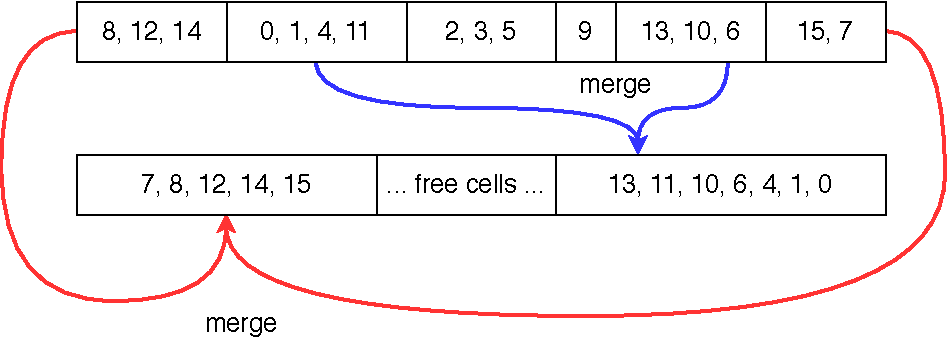
\includegraphics[scale=0.8]{img/nature-merge-sort}
 \caption{Nature merge sort}
 \label{fig:nature-merge-sort}
\end{figure}

Figure \ref{fig:nature-merge-sort} illustrates this idea. We starts the algorithm by scanning
from both ends, finding the longest non-decreasing sub sequences respectively. After that,
these two sub sequences are merged to the working area. The merged result starts from beginning.
Next we repeat this step, which goes on scanning toward the center of the original sequence.
This time we merge the two ordered sub sequences to the right hand of the working area toward
the left. Such setup is easy for the next round of scanning. When all the elements
in the original sequence have been scanned and merged to the target, we switch to use the
elements stored in the working area for sorting, and use the previous sequence as new working area.
Such switching happens repeatedly in each round. Finally, we copy all elements from the
working area to the original array if necessary.

The only question left is when this algorithm stops. The answer is that when we start
a new round of scanning, and find that the longest non-decreasing sub list spans to the
end, which means the whole list is ordered, the sorting is done.

Because this kind of merge sort proceeds the target sequence in two ways, and uses the
nature ordering of sub sequences, it's named {\em nature two-way merge sort}. In order
to realize it, some carefulness must be paid. Figure \ref{fig:nature-msort-invariant}
shows the invariant during the nature merge sort. At anytime, all elements before marker
$a$ and after marker $d$ have been already scanned and merged. We are trying to
span the non-decreasing sub sequence $[a, b)$ as long as possible, at the same time,
we span the sub sequence from right to left to span $[c, d)$ as long as possible as well.
The invariant for the working area is shown in the second row. All elements before
$f$ and after $r$ have already been processed (Note that they may contain several
ordered sub sequences). For the odd times (1, 3, 5, ...), we merge $[a, b)$ and $[c, d)$
from $f$ toword right; while for the even times (2, 4, 6, ...), we merge the two
sorted sub sequences after $r$ toward left.

\begin{figure}[htbp]
 \centering
 \includegraphics[scale=0.8]{img/nature-msort-invariant}
 \caption{Invariant during nature merge sort}
 \label{fig:nature-msort-invariant}
\end{figure}

For imperative realization, the sequence is represented by array. Before sorting starts,
we duplicate the array to create a working area. The pointers $a, b$ are initialized to
point the left most position, while $c, d$ point to the right most position. Pointer $f$
starts by pointing to the front of the working area, and $r$ points to the rear
position.

\begin{algorithmic}[1]
\Function{Sort}{$A$}
  \If{$|A| > 1$}
    \State $n \gets |A|$
    \State $B \gets$ \Call{Create-Array}{$n$}  \Comment{Create the working area}
    \Loop
      \State $[a, b) \gets [1, 1)$
      \State $[c, d) \gets [n+1, n+1)$
      \State $f \gets 1, r \gets n$ \Comment{front and rear pointers to the working area}
      \State $t \gets $ False \Comment{merge to front or rear}
      \While{$b < c$} \Comment{There are still elements for scan}
        \Repeat \Comment{Span $[a, b)$}
          \State $b \gets b + 1$
        \Until{$b \geq c \lor A[b] < A[b-1]$}

        \Repeat \Comment{Span $[c, d)$}
          \State $c \gets c - 1$
        \Until{$c \leq b \lor A[c-1] < A[c]$}

        \If{$c < b$} \Comment{Avoid overlap}
          \State $c \gets b$
        \EndIf

        \If{$b - a \geq n$} \Comment{Done if $[a, b)$ spans to the whole array}
          \State \Return $A$
        \EndIf

        \If{$t$} \Comment{merge to front}
          \State $f \gets$ \Call{Merge}{$A, [a, b), [c, d), B, f, 1$}
        \Else \Comment{merge to rear}
          \State $r \gets$ \Call{Merge}{$A, [a, b), [c, d), B, r, -1$}
        \EndIf
        \State $a \gets b, d \gets c$
        \State $t \gets \lnot t$ \Comment{Switch the merge direction}
      \EndWhile
      \State \textproc{Exchange} $A \leftrightarrow B$ \Comment{Switch working area}
    \EndLoop
  \EndIf
  \State \Return $A$
\EndFunction
\end{algorithmic}

The merge algorithm is almost as same as before except that we need pass a parameter
to indicate the direction for merging.

\begin{algorithmic}[1]
\Function{Merge}{$A, [a, b), [c, d), B, w, \Delta$}
  \While{$a < b \land c < d$}
    \If{$A[a] < A[d-1]$}
      \State $B[w] \gets A[a]$
      \State $a \gets a + 1$
    \Else
      \State $B[w] \gets A[d-1]$
      \State $d \gets d - 1$
    \EndIf
    \State $w \gets w + \Delta$
  \EndWhile
  \While{$a < b$}
    \State $B[w] \gets A[a]$
    \State $a \gets a + 1$
    \State $w \gets w + \Delta$
  \EndWhile
  \While{$c < d$}
    \State $B[w] \gets A[d-1]$
    \State $d \gets d - 1$
    \State $w \gets w + \Delta$
  \EndWhile
  \State \Return $w$
\EndFunction
\end{algorithmic}

The following ANSI C program implements this two-way nature merge sort algorithm. Note that it
doesn't release the allocated working area explicitly.

\lstset{language=C}
\begin{lstlisting}
int merge(Key* xs, int a, int b, int c, int d, Key* ys, int k, int delta) {
    for(; a < b && c < d; k += delta )
        ys[k] = xs[a] < xs[d-1] ? xs[a++] : xs[--d];
    for(; a < b; k += delta)
        ys[k] = xs[a++];
    for(; c < d; k += delta)
        ys[k] = xs[--d];
    return k;
}

Key* sort(Key* xs, Key* ys, int n) {
    int a, b, c, d, f, r, t;
    if(n < 2)
        return xs;
    for(;;) {
        a = b = 0;
        c = d = n;
        f = 0;
        r = n-1;
        t = 1;
        while(b < c) {
            do {      /* span [a, b) as much as possible */
                ++b;
            } while( b < c && xs[b-1] <= xs[b] );
            do{      /* span [c, d) as much as possible */
                --c;
            } while( b < c && xs[c] <= xs[c-1] );
            if( c < b )
                c = b;   /* eliminate overlap if any */
            if( b - a >= n)
                return xs;          /* sorted */
            if( t )
                f = merge(xs, a, b, c, d, ys, f, 1);
            else
                r = merge(xs, a, b, c, d, ys, r, -1);
            a = b;
            d = c;
            t = !t;
        }
        swap(&xs, &ys);
    }
    return xs; /*can't be here*/
}
\end{lstlisting}

The performance of nature merge sort depends on the actual ordering of the sub arrays. However, it in fact performs
well even in the worst case. Suppose that we are unlucky when scanning the array, that the length of the non-decreasing
sub arrays are always 1 during the first round scan. This leads to the result working area with merged ordered sub
arrays of length 2. Suppose that we are unlucky again in the second round of scan, however, the previous results
ensure that the non-decreasing sub arrays in this round are no shorter than 2, this time, the working area will
be filled with merged ordered sub arrays of length 4, ... Repeat this we get the length of the non-decreasing sub arrays
doubled in every round, so there are at most $O(\lg n)$ rounds, and in every round we scanned all the elements.
The overall performance for this worst case is bound to $O(n \lg n)$. We'll go back to this interesting phenomena
in the next section about bottom-up merge sort.

In purely functional settings however, it's not sensible to scan list from both ends since the underlying data
structure is singly linked-list. The nature merge sort can be realized in another approach.

Observe that the list to be sorted is consist of several non-decreasing sub lists, that we can pick every two
of such sub lists and merge them to a bigger one. We repeatedly pick and merge, so that the number of the
non-decreasing sub lists halves continuously and finally there is only one such list, which is the sorted
result. This idea can be formalized in the following equation.

\be
sort(L) = sort'(group(L))
\ee

Where function $group(L)$ groups the elements in the list into non-decreasing sub lists. This function can be described like
below, the first two are trivial edge cases.

\begin{itemize}
\item If the list is empty, the result is a list contains an empty list;
\item If there is only one element in the list, the result is a list contains a singleton list;
\item Otherwise, The first two elements are compared, if the first one is less than or equal to the second,
it is linked in front of the first sub list of the recursive grouping result; or a singleton list contains
the first element is set as the first sub list before the recursive result.
\end{itemize}

\be
group(L) =  \left \{
  \begin{array}
  {r@{\quad:\quad}l}
  \{ L \} & |L| \leq 1 \\
  \{ \{ l_1 \} \cup L_1, L_2, ... \} & l_1 \leq l_2, \{ L_1, L_2, ...\} = group(L') \\
  \{ \{ l_1 \}, L_1, L_2, ... \} & otherwise
  \end{array}
\right.
\ee

It's quite possible to abstract the grouping criteria as a parameter to develop a generic grouping function,
for instance, as the following Haskell code \footnote{There is a `groupBy' function provided in
the Haskell standard library 'Data.List'. However, it doesn't fit here, because it accepts an equality
testing function as parameter, which must satisfy the properties of reflexive, transitive, and
symmetric. but what we use here, the less-than or equal to operation doesn't conform to symetric. Refer
to appendix A of this book for detail.}.

\lstset{language=Haskell}
\begin{lstlisting}
groupBy' :: (a->a->Bool) ->[a] ->[[a]]
groupBy' _ [] = [[]]
groupBy' _ [x] = [[x]]
groupBy' f (x:xs@(x':_)) | f x x' = (x:ys):yss
                         | otherwise = [x]:r
  where
    r@(ys:yss) = groupBy' f xs
\end{lstlisting}

Different from the $sort$ function, which sorts a list of elements, function $sort'$ accepts a list of
sub lists which is the result of grouping.

\be
sort'(\mathbb{L}) = \left \{
  \begin{array}
  {r@{\quad:\quad}l}
  \phi & \mathbb{L} = \phi \\
  L_1 & \mathbb{L} = \{ L_1 \} \\
  sort'(mergePairs(\mathbb{L})) & otherwise
  \end{array}
\right.
\ee

The first two are the trivial edge cases. If the list to be sorted is empty, the result is obviously empty;
If it contains only one sub list, then we are done. We need just extract this single sub list as result;
For the recursive case, we call a function $mergePairs$ to merge every two sub lists, then recursively call
$sort'$.

The next undefined function is $mergePairs$, as the name indicates, it repeatedly merges pairs of non-decreasing
sub lists into bigger ones.

\be
mergePairs(L) = \left \{
  \begin{array}
  {r@{\quad:\quad}l}
  L & |L| \leq 1 \\
  \{ merge(L_1, L_2) \} \cup mergePairs(L'') & otherwise
  \end{array}
\right.
\ee

When there are less than two sub lists in the list, we are done; otherwise, we merge the first two sub lists $L_1$ and $L_2$,
and recursively merge the rest of pairs in $L''$. The type of
the result of $mergePairs$ is list of lists, however, it will be flattened by $sort'$ function finally.

The $merge$ function is as same as before. The complete example Haskell program is given as below.

\lstset{language=Haskell}
\begin{lstlisting}
mergesort = sort' . groupBy' (<=)

sort' [] = []
sort' [xs] = xs
sort' xss = sort' (mergePairs xss) where
  mergePairs (xs:ys:xss) = merge xs ys : mergePairs xss
  mergePairs xss = xss
\end{lstlisting}

Alternatively, observing that we can first pick two sub lists, merge them to an intermediate result, then repeatedly
pick next sub list, and merge to this ordered result we've gotten so far until all the rest sub lists are merged.
This is a typical folding algorithm as introduced in appendix A.

\be
sort(L) = fold(merge, \phi, group(L))
\ee

Translate this version to Haskell yields the folding version.

\lstset{language=Haskell}
\begin{lstlisting}
mergesort' = foldl merge [] . groupBy' (<=)
\end{lstlisting}

\begin{Exercise}
\begin{itemize}
  \item Is the nature merge sort algorithm realized by folding is equivalent with the one by using $mergePairs$ in terms
of performance? If yes, prove it; If not, which one is faster?
\end{itemize}
\end{Exercise}

\section{Bottom-up merge sort}
\index{Merge Sort!Bottom-up merge sort}
The worst case analysis for nature merge sort raises an interesting topic, instead of realizing merge sort in
top-down manner, we can develop a bottom-up version. The great advantage is that, we needn't do book keeping
any more, so the algorithm is quite friendly for purely iterative implementation.

The idea of bottom-up merge sort is to turn the sequence to be sorted into $n$ small sub sequences each contains
only one element. Then we merge every two of such small sub sequences, so that we get $\frac{n}{2}$ ordered
sub sequences each with length 2; If $n$ is odd number, we left the last singleton sequence untouched.
We repeatedly merge these pairs, and finally we get the sorted result. Knuth names this variant as
`straight two-way merge sort' \cite{TAOCP}. The bottom-up merge sort is illustrated in figure \ref{fig:bottom-up-msort}

\begin{figure}[htbp]
 \centering
 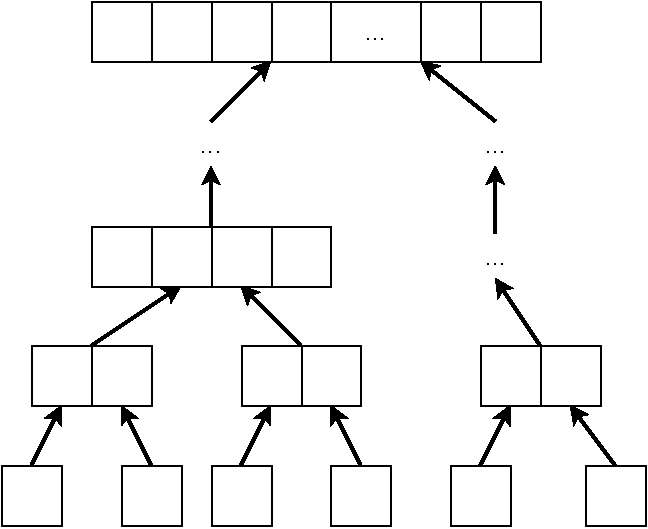
\includegraphics[scale=0.6]{img/bottom-up-msort}
 \caption{Bottom-up merge sort}
 \label{fig:bottom-up-msort}
\end{figure}

Different with the basic version and even-odd version, we needn't explicitly split the list to be sorted
in every recursion. The whole list is split into $n$ singletons at the very beginning, and we merge these
sub lists in the rest of the algorithm.

\be
sort(L) = sort'(wraps(L))
\ee

\be
wraps(L) = \left \{
  \begin{array}
  {r@{\quad:\quad}l}
  \phi & L = \phi \\
  \{ \{l_1\} \} \cup wraps(L') & otherwise
  \end{array}
\right.
\ee

Of course $wraps$ can be implemented by using mapping as introduced in appendix A.

\be
sort(L) = sort'(map(\lambda_x \cdot \{ x \}, L))
\ee

We reuse the function $sort'$ and $mergePairs$ which are defined in section of nature merge sort. They
repeatedly merge pairs of sub lists until there is only one.

Implement this version in Haskell gives the following example code.

\lstset{language=Haskell}
\begin{lstlisting}
sort = sort' . map (\x->[x])
\end{lstlisting}

This version is based on what Okasaki presented in \cite{okasaki-book}. It is quite similar to the nature merge sort
only differs in the way of grouping. Actually, it can be deduced as a special case (the worst case) of
nature merge sort by the following equation.

\be
sort(L)= sort'(groupBy(\lambda_{x, y} \cdot False, L))
\ee

That instead of spanning the non-decreasing sub list as long as possible, the predicate always evaluates to false,
so the sub list spans only one element.

Similar with nature merge sort, bottom-up merge sort can also be defined by folding. The detailed implementation
is left as exercise to the reader.

Observing the bottom-up sort, we can find it's in tail-recursion call manner, thus it's quite easy
to translate into purely iterative algorithm without any recursion.

\begin{algorithmic}[1]
\Function{Sort}{$A$}
  \State $B \gets \phi$
  \For{$\forall a \in A$}
    \State $B \gets$ \Call{Append}{$\{ a \}$}
  \EndFor
  \State $N \gets |B|$
  \While{$N > 1$}
    \For{$i \gets $ from $1$ to $\lfloor \frac{N}{2} \rfloor$}
      \State $B[i] \gets$ \Call{Merge}{$B[2i -1], B[2i]$}
    \EndFor
    \If{\Call{Odd}{$N$}}
      \State $B[\lceil \frac{N}{2} \rceil] \gets B[N]$
    \EndIf
    \State $N \gets \lceil \frac{N}{2} \rceil$
  \EndWhile
  \If{$B = \phi$}
    \State \Return $\phi$
  \EndIf
  \State \Return $B[1]$
\EndFunction
\end{algorithmic}

The following example Python program implements the purely iterative bottom-up merge sort.

\lstset{language=Python}
\begin{lstlisting}
def mergesort(xs):
    ys = [[x] for x in xs]
    while len(ys) > 1:
        ys.append(merge(ys.pop(0), ys.pop(0)))
    return [] if ys == [] else ys.pop()

def merge(xs, ys):
    zs = []
    while xs != [] and ys !=[]:
        zs.append(xs.pop(0) if xs[0] < ys[0] else ys.pop(0))
    return zs + (xs if xs !=[] else ys)
\end{lstlisting}

The Python implementation combines multiple rounds of merging by consuming
the pair of lists on the head, and appending the merged result to the tail. This greatly simply
the logic of handling odd sub lists case as shown in the above pseudo code.

\begin{Exercise}
\begin{itemize}
\item Implement the functional bottom-up merge sort by using folding.
\item Implement the iterative bottom-up merge sort only with array indexing. Don't use any library
supported tools, such as list, vector etc.
\end{itemize}
\end{Exercise}

\section{Parallelism}
\index{Parallel merge sort}
\index{Parallel quick sort}
We mentioned in the basic version of quick sort, that the two sub sequences can be sorted in
parallel after the divide phase finished. This strategy is also applicable for merge sort.
Actually, the parallel version quick sort and morege sort, do not only distribute
the recursive sub sequences sorting into two parallel processes, but divide the sequences into
$p$ sub sequences, where $p$ is the number of processors. Idealy, if we can achieve
sorting in $T'$ time with parallelism, which satisifies $O(n \lg n) = p T'$. We say it
is linear speed up, and the algorithm is parallel optimal.

However, a straightforward parallel extension to the sequential quick sort algorithm
which samples several pivots, divides $p$ sub sequences, and independently
sorts them in parallel, isn't optimal. The bottleneck exists in the
divide phase, which we can only achieve $O(n)$ time in average case.

The straightforward parallel extension to merge sort, on the other hand, block
at the merge phase. Both parallel merge sort and quick sort in practice need
good designs in order to achieve the optimal speed up. Actually, the divide and
conquer nature makes merge sort and quick sort relative easy for parallelisim.
Richard Cole found the $O(\lg n)$ parallel merge sort algorithm with $n$ processors
in 1986 in \cite{para-msort}.

Parallelism is a big and complex
topic which is out of the scope of this elementary book. Readers can refer to
\cite{para-msort} and \cite{para-qsort} for details.

\section{Short summary}
In this chapter, two popular divide and conquer sorting methods, quick sort and merge sort are introduced.
Both of them meet the upper performance limit of the comparison based sorting algorithms $O(n \lg n)$.
Sedgewick said that quick sort is the greatest algorithm invented in the 20th century. Almost
all programming environments adopt quick sort as the default sorting tool. As time goes on,
some environments, especially those manipulate abstract sequence which is dynamic and not based on
pure array switch to merge sort as the general purpose sorting tool\footnote{Actually, most of
them are kind of hybrid sort, balanced with insertion sort to achieve good performance when the
sequence is short}.

The reason for this interesting phenomena can be partly explained by the treatment in this chapter.
That quick sort performs perfectly in most cases, it needs fewer swapping than most other algorithms.
However, the quick sort algorithm is based on swapping, in purely functional settings, swapping isn't
the most efficient way due to the underlying data structure is singly linked-list, but not vectorized
array. Merge sort, on the other hand, is friendly in such environment, as it costs constant spaces,
and the performance can be ensured even in the worst case of quick sort, while the latter downgrade
to quadratic time. However, merge sort doesn't performs as well as quick sort in purely imperative
settings with arrays. It either needs extra spaces for merging, which is sometimes unreasonable, for
example in embedded system with limited memory, or causes many overhead swaps by in-place workaround.
In-place merging is till an active research area.

Although the title of this chapter is `quick sort vs. merge sort', it's not the case that one
algorithm has nothing to do with the other. Quick sort can be viewed as the optimized version of
tree sort as explained in this chapter. Similarly, merge sort can also be deduced from tree sort
as shown in \cite{sort-deriving}.

There are many ways to categorize sorting algorithms, such as in \cite{TAOCP}. One way is to
from the point of view of easy/hard partition, and easy/hard merge \cite{algo-fp}.

Quick sort, for example, is quite easy for merging, because all the elements in the sub
sequence before the pivot are no greater than any one after the pivot. The merging for
quick sort is actually trivial sequence concatenation.

Merge sort, on the other hand, is more complex in merging than quick sort. However, it's
quite easy to divide no matter what concrete divide method is taken:
simple divide at the middle point, even-odd splitting, nature splitting, or bottom-up
straight splitting. Compare to merge sort, it's more difficult for quick sort to
achieve a perfect dividing. We show that in theory, the worst case can't be completely
avoided, no matter what engineering practice is taken, median-of-three, random quick sort,
3-way partition etc.

We've shown some elementary sorting algorithms in this book till this chapter, including
insertion sort, tree sort, selection sort, heap sort, quick sort and merge sort. Sorting
is still a hot research area in computer science. At the time when this chapter is written,
people are challenged by the buzz word `big data', that the traditional convenient method
can't handle more and more huge data within reasonable time and resources.
Sorting a sequence of hundreds of Gigabytes becomes a routine in some fields.

\begin{Exercise}
  \begin{itemize}
    \item Design an algorithm to create binary search tree by using merge sort strategy.
  \end{itemize}
\end{Exercise}

\ifx\wholebook\relax\else

\begin{thebibliography}{99}

\bibitem{TAOCP}
Donald E. Knuth. ``The Art of Computer Programming, Volume 3: Sorting and Searching (2nd Edition)''. Addison-Wesley Professional; 2 edition (May 4, 1998) ISBN-10: 0201896850 ISBN-13: 978-0201896855

\bibitem{CLRS}
Thomas H. Cormen, Charles E. Leiserson, Ronald L. Rivest and Clifford Stein.
``Introduction to Algorithms, Second Edition''. ISBN:0262032937. The MIT Press. 2001

\bibitem{qsort-impl}
Robert Sedgewick. ``Implementing quick sort programs''. Communication of ACM. Volume 21, Number 10. 1978. pp.847 - 857.

\bibitem{Bentley}
Jon Bentley. ``Programming pearls, Second Edition''. Addison-Wesley Professional; 1999. ISBN-13: 978-0201657883

\bibitem{3-way-part}
Jon Bentley, Douglas McIlroy. ``Engineering a sort function''. Software Practice and experience VOL. 23(11), 1249-1265 1993.

\bibitem{opt-qs}
Robert Sedgewick, Jon Bentley. ``Quicksort is optimal''. \url{http://www.cs.princeton.edu/~rs/talks/QuicksortIsOptimal.pdf}

\bibitem{fp-pearls}
Richard Bird. ``Pearls of functional algorithm design''. Cambridge University Press. 2010. ISBN, 1139490605, 9781139490603

\bibitem{algo-fp}
Fethi Rabhi, Guy Lapalme. ``Algorithms: a functional programming approach''. Second edition. Addison-Wesley, 1999. ISBN: 0201-59604-0

\bibitem{slpj}
Simon Peyton Jones. ``The Implementation of functional programming languages''. Prentice-Hall International, 1987. ISBN: 0-13-453333-X

\bibitem{msort-in-place}
Jyrki Katajainen, Tomi Pasanen, Jukka Teuhola. ``Practical in-place mergesort''. Nordic Journal of Computing, 1996.

\bibitem{okasaki-book}
Chris Okasaki. ``Purely Functional Data Structures''. Cambridge university press, (July 1, 1999), ISBN-13: 978-0521663502

\bibitem{sort-deriving}
Jos\`{e} Bacelar Almeida and Jorge Sousa Pinto. ``Deriving Sorting Algorithms''. Technical report, Data structures and Algorithms. 2008.

\bibitem{para-msort}
Cole, Richard (August 1988). ``Parallel merge sort''. SIAM J. Comput. 17 (4): 770-785. doi:10.1137/0217049. (August 1988)

\bibitem{para-qsort}
Powers, David M. W. ``Parallelized Quicksort and Radixsort with Optimal Speedup'', Proceedings of International Conference on Parallel Computing Technologies. Novosibirsk. 1991.

\bibitem{wiki-qs}
Wikipedia. ``Quicksort''. \url{https://en.wikipedia.org/wiki/Quicksort}

\bibitem{wiki-sweak-order}
Wikipedia. ``Strict weak order''. \url{https://en.wikipedia.org/wiki/Strict_weak_order}

\bibitem{wiki-total-order}
Wikipedia. ``Total order''. \url{http://en.wokipedia.org/wiki/Total_order}

\bibitem{wiki-harmonic}
Wikipedia. ``Harmonic series (mathematics)''. \url{https://en.wikipedia.org/wiki/Harmonic_series_(mathematics)}

\end{thebibliography}

\expandafter\enddocument
\fi
